% Incluyendo el preambulo de LaTeX para configurar los paquetes que se vayan usando
% Configuracion inicial del documento
\documentclass[a4paper]{article}

% Paquetes utilizados
\usepackage[utf8]{inputenc}
\usepackage[spanish, es-tabla]{babel}
\usepackage{float}
\usepackage{graphicx}
\usepackage{multirow}
\usepackage{circuitikz}

% Paquetes de matematica
\usepackage{amsmath}
\usepackage{amssymb}
\usepackage{steinmetz}

% Paquetes para excel
\usepackage{csvsimple}

% Configuracion del informe
\setlength{\parindent}{0pt}
\setcounter{secnumdepth}{0}

\usepackage[a4paper, 
    includehead, 
    footskip=7mm, 
    headsep=6mm, 
    headheight=4.8mm,
    top=25mm, bottom=25mm, left=25mm, right=25mm]{geometry}

\usepackage{hyperref}
\hypersetup{
    colorlinks=true,
    linkcolor=blue,
    filecolor=magenta,      
    urlcolor=blue,
    citecolor=blue,    
}

% Abrir y crear el documento, llamar a cada uno de los ejercicios
\begin{document}

    % Crear y configurar el titulo/caratula del informe
    \title{
        \normalfont \normalsize \textsc{Instituto Tecnol\'ogico de Buenos Aires} \\ [25pt]
        \huge Trabajo Pr\'actico Nº 2 \\
        \author{
            \\Grupo 1:\\\\Galdeman, Agust\'in Ignacio\\Gaytan, Joaqu\'in Oscar\\Kammann, Lucas\\Maselli, Carlos Javier\\ \\ \\ \\
            Profesores: \\\\ Cossutta, Pablo Mart\'in\\Weill, Mar\'ia Alejandra\\Salvati, Mat\'ias Dami\'an \\ \\ \\ 
        } 
        \text{Laboratorio de Electr\'onica - 2019}
    }
    \pagenumbering{arabic}

    \maketitle
    \newpage

    % Crear indice del informe
    \tableofcontents

    % Incluyendo los ejercicios realizados
    \newpage
    


\section{Caracterizaci\'on de componentes pasivos}
En esta secci\'on se analiza el comportamiento de los componentes pasivos en funci\'on de la frecuencia de operaci\'on, en particular de un capacitor y un inductor.
Para dicho an\'alisis se realiza un barrido en frecuencias desde $10Hz$ a $10MHz$.

\subsection{Medici\'on del capacitor}
Para la medici\'on se utiliza un capacitor de $22nF$ de film y se configura el analizador de impedancias en modelo paralelo para medir fase y admitancia. En este caso, debido a las caracter\'isticas particulares del componente, no es posible realizar el barrido de frecuencias completo.
\subsubsection{Resultados}
Se muestran en la Tabla \ref{tab:Med_CAP}  los resultados obtenidos de las mediciones y en la Figura \ref{fig:Med_CAP} los respectivos  gr\'aficos realizados a partir de estas.

\begin{table}[H]
    \centering
    \resizebox{0.5\textwidth}{!}{%
        \begin{tabular}{ccccc}
            \hline
            \begin{tabular}[c]{@{}c@{}}Frecuencia\\   (Hz)\end{tabular} & Capacidad (F) & \begin{tabular}[c]{@{}c@{}}Factor de\\   disipación\end{tabular} & Admitancia (s) & Fase ($^\circ$) \\ \hline
            5 & 2.20E-08 & 0.006 & 6.80E-07 & 89.5 \\
            10 & 2.19E-08 & 0.006 & 1.38E-06 & 89.9 \\
            20 & 2.20E-08 & 0 & 2.76E-06 & 90 \\
            100 & 2.19E-08 & 0.0012 & 1.38E-05 & 89.93 \\
            300 & 2.19E-08 & 0.0025 & 4.13E-05 & 89.86 \\
            1000 & 2.19E-08 & 0.0039 & 1.37E-04 & 89.78 \\
            3000 & 2.18E-08 & 0.0064 & 4.10E-04 & 89.64 \\
            10000 & 2.17E-08 & 0.0086 & 1.36E-03 & 89.51 \\
            30000 & 2.15E-08 & 0.0124 & 4.05E-03 & 89.29 \\
            80000 & 2.13E-08 & 0.0157 & 1.07E-02 & 89.1 \\
            100000 & 2.13E-08 & 0.0165 & 1.34E-02 & 89.06 \\
            150000 & 2.12E-08 & 0.018 & 2.00E-02 & 88.97 \\
            200000 & 2.11E-08 & 0.0191 & 2.66E-02 & 88.91 \\
            300000 & 2.11E-08 & 0.0211 & 3.97E-02 & 88.79 \\
            400000 & 2.10E-08 & 0.0228 & 5.28E-02 & 88.69 \\
            500000 & 2.10E-08 & 0.0245 & 6.60E-02 & 88.6 \\
            600000 & 2.10E-08 & 0.0262 & 7.91E-02 & 88.5 \\
            700000 & 2.10E-08 & 0.0279 & 9.24E-02 & 88.4 \\
            750000 & 2.10E-08 & 0.0287 & 9.90E-02 & 88.35 \\
            780000 & 2.10E-08 & 0.0292 & 1.03E-01 & 88.32 \\
            800000 & 2.10E-08 & 0.0296 & 1.06E-01 & 88.31 \\
            825000 & 2.10E-08 & 0.03 & 1.09E-01 & 88.28 \\
            850000 & 2.10E-08 & 0.0305 & 1.12E-01 & 88.25 \\
            900000 & 2.11E-08 & 0.0313 & 1.19E-01 & 88.18 \\
            1000000 & 2.11E-08 & 0.033 & 0.133 & 88.1 \\
            2000000 & 2.19E-08 & 0.052 & 0.276 & 87 \\
            3000000 & 2.36E-08 & 0.077 & 0.447 & 85.6 \\
            4000000 & 2.66E-08 & 0.112 & 0.673 & 83.6 \\
            5000000 & 3.18E-08 & 0.166 & 1.012 & 80.6 \\
             \hline
        \end{tabular}%
    }
    \caption{Mediciones del capacitor}
    \label{tab:Med_CAP}
\end{table}

\begin{figure}[H]
    \centering
    \resizebox{\textwidth}{!}{
        \begin{tabular}{c c}
            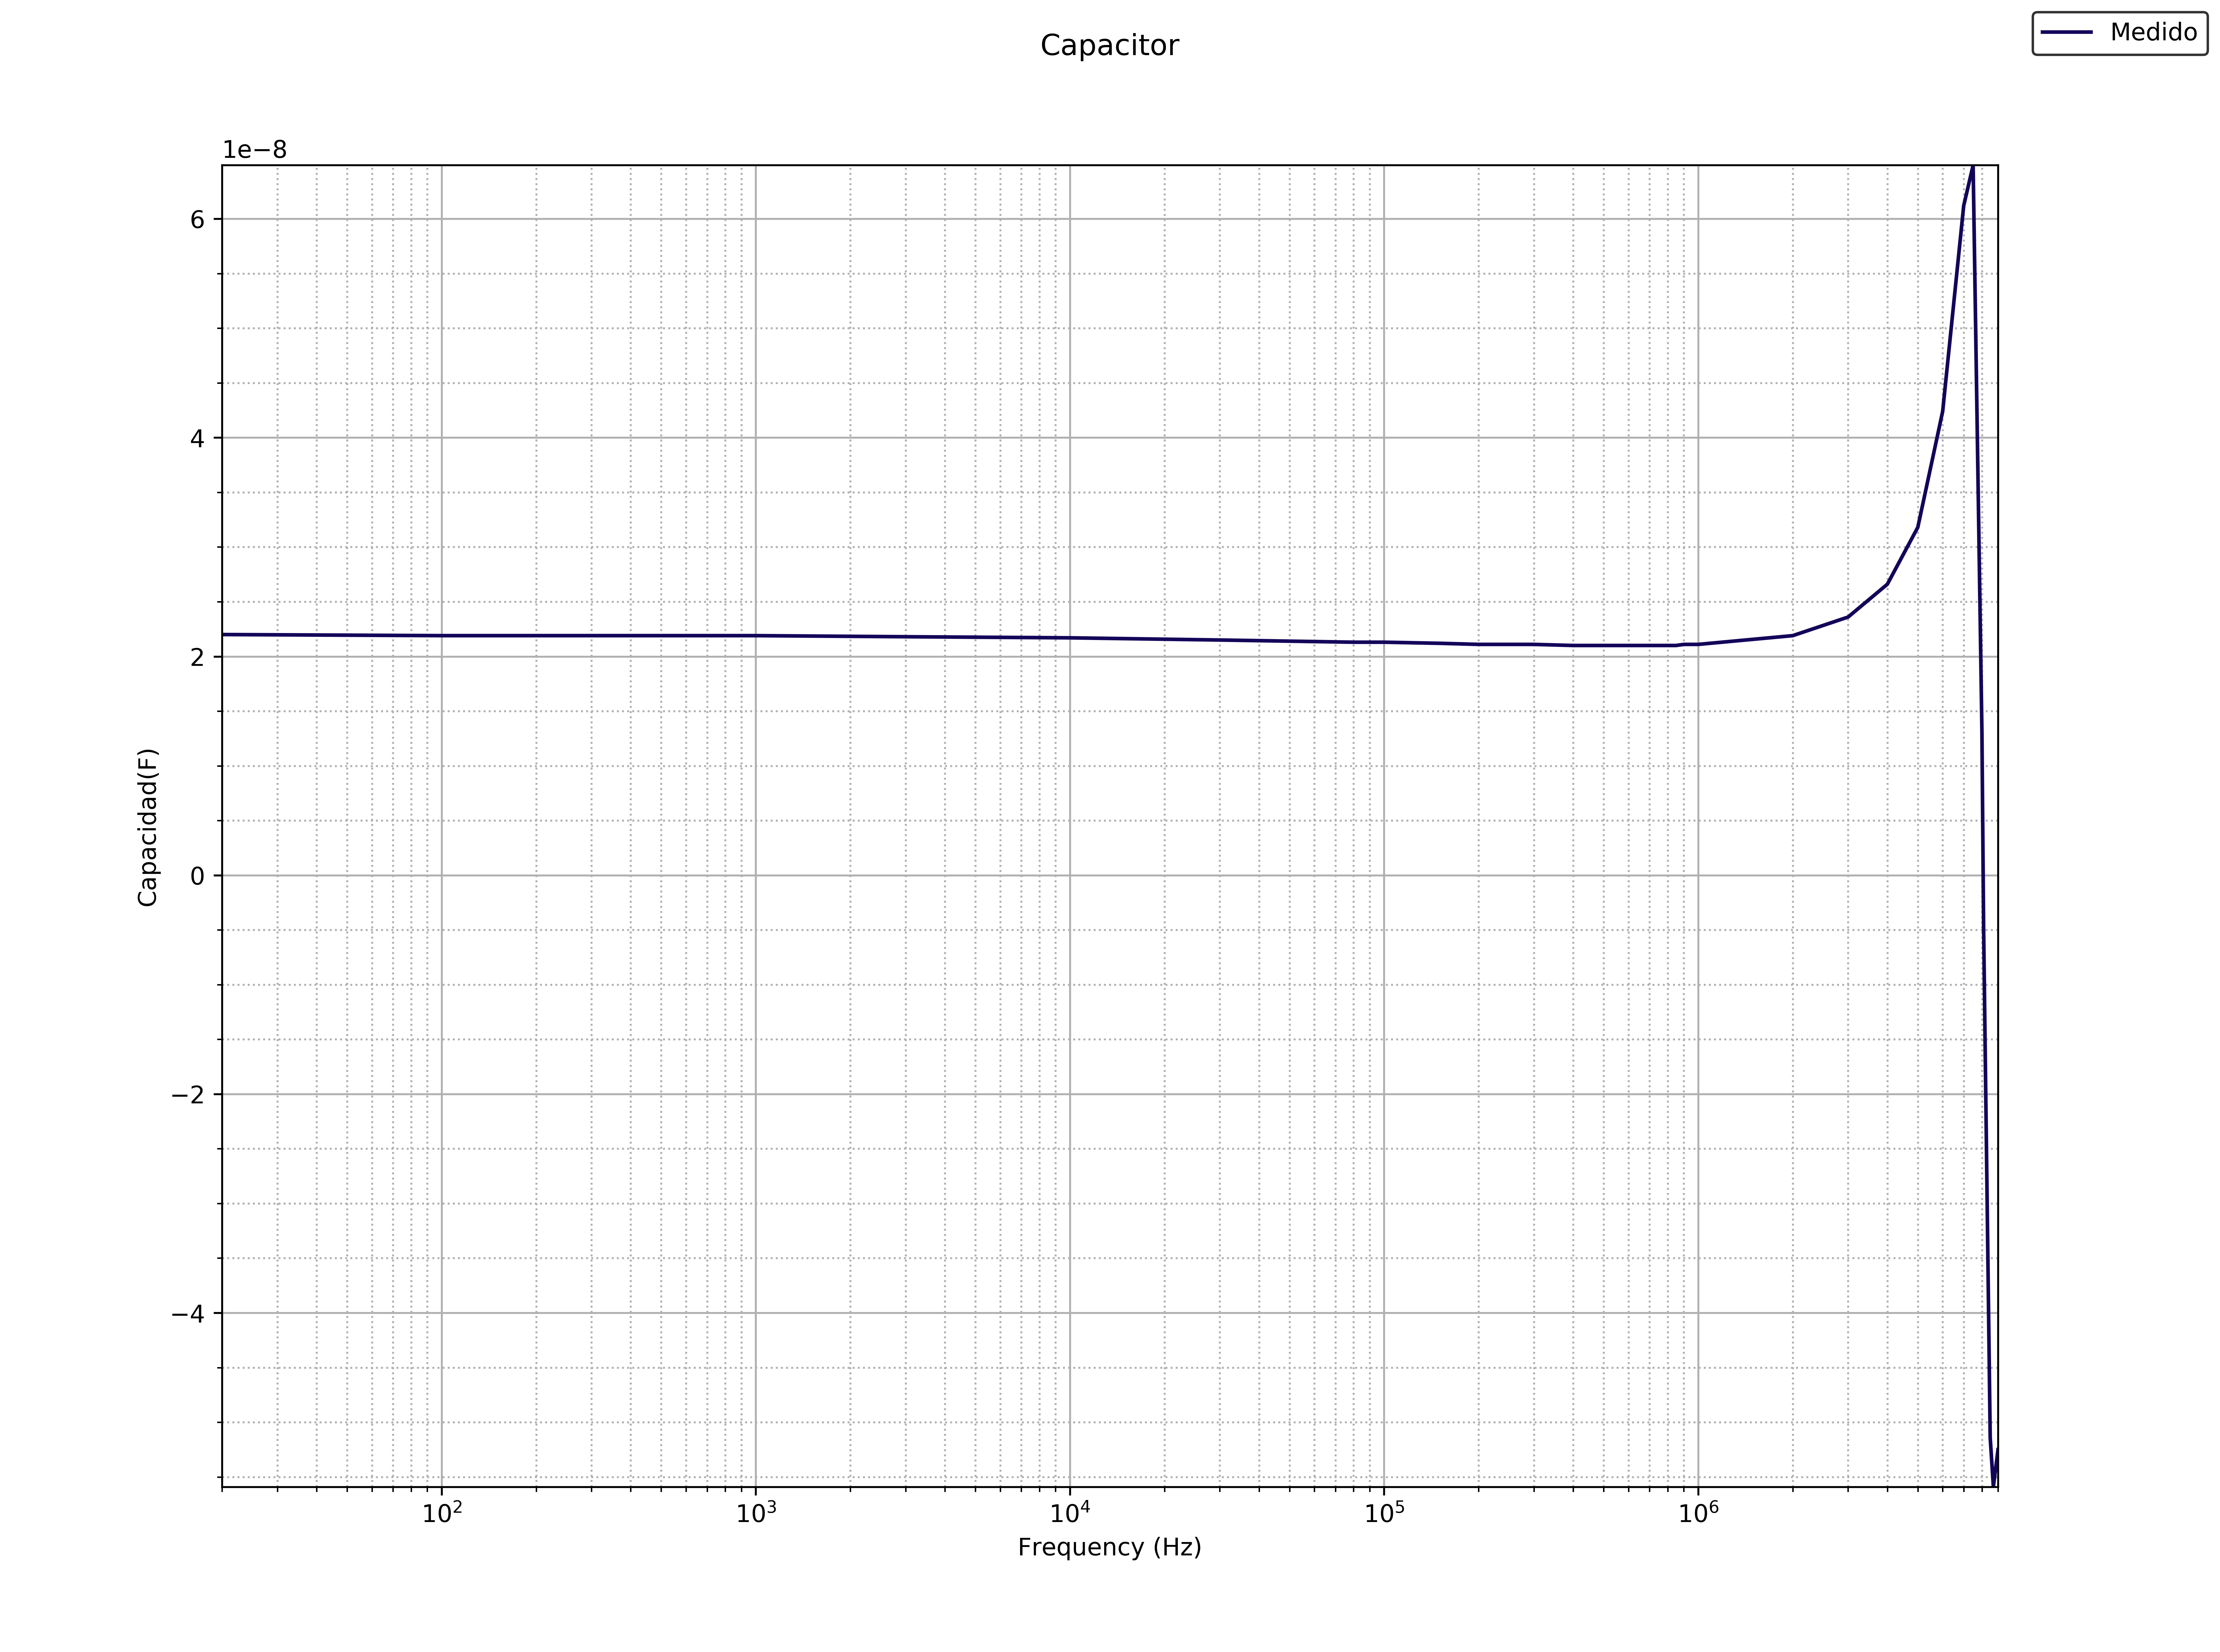
\includegraphics{Recursos/capacidad_medida.png}&
            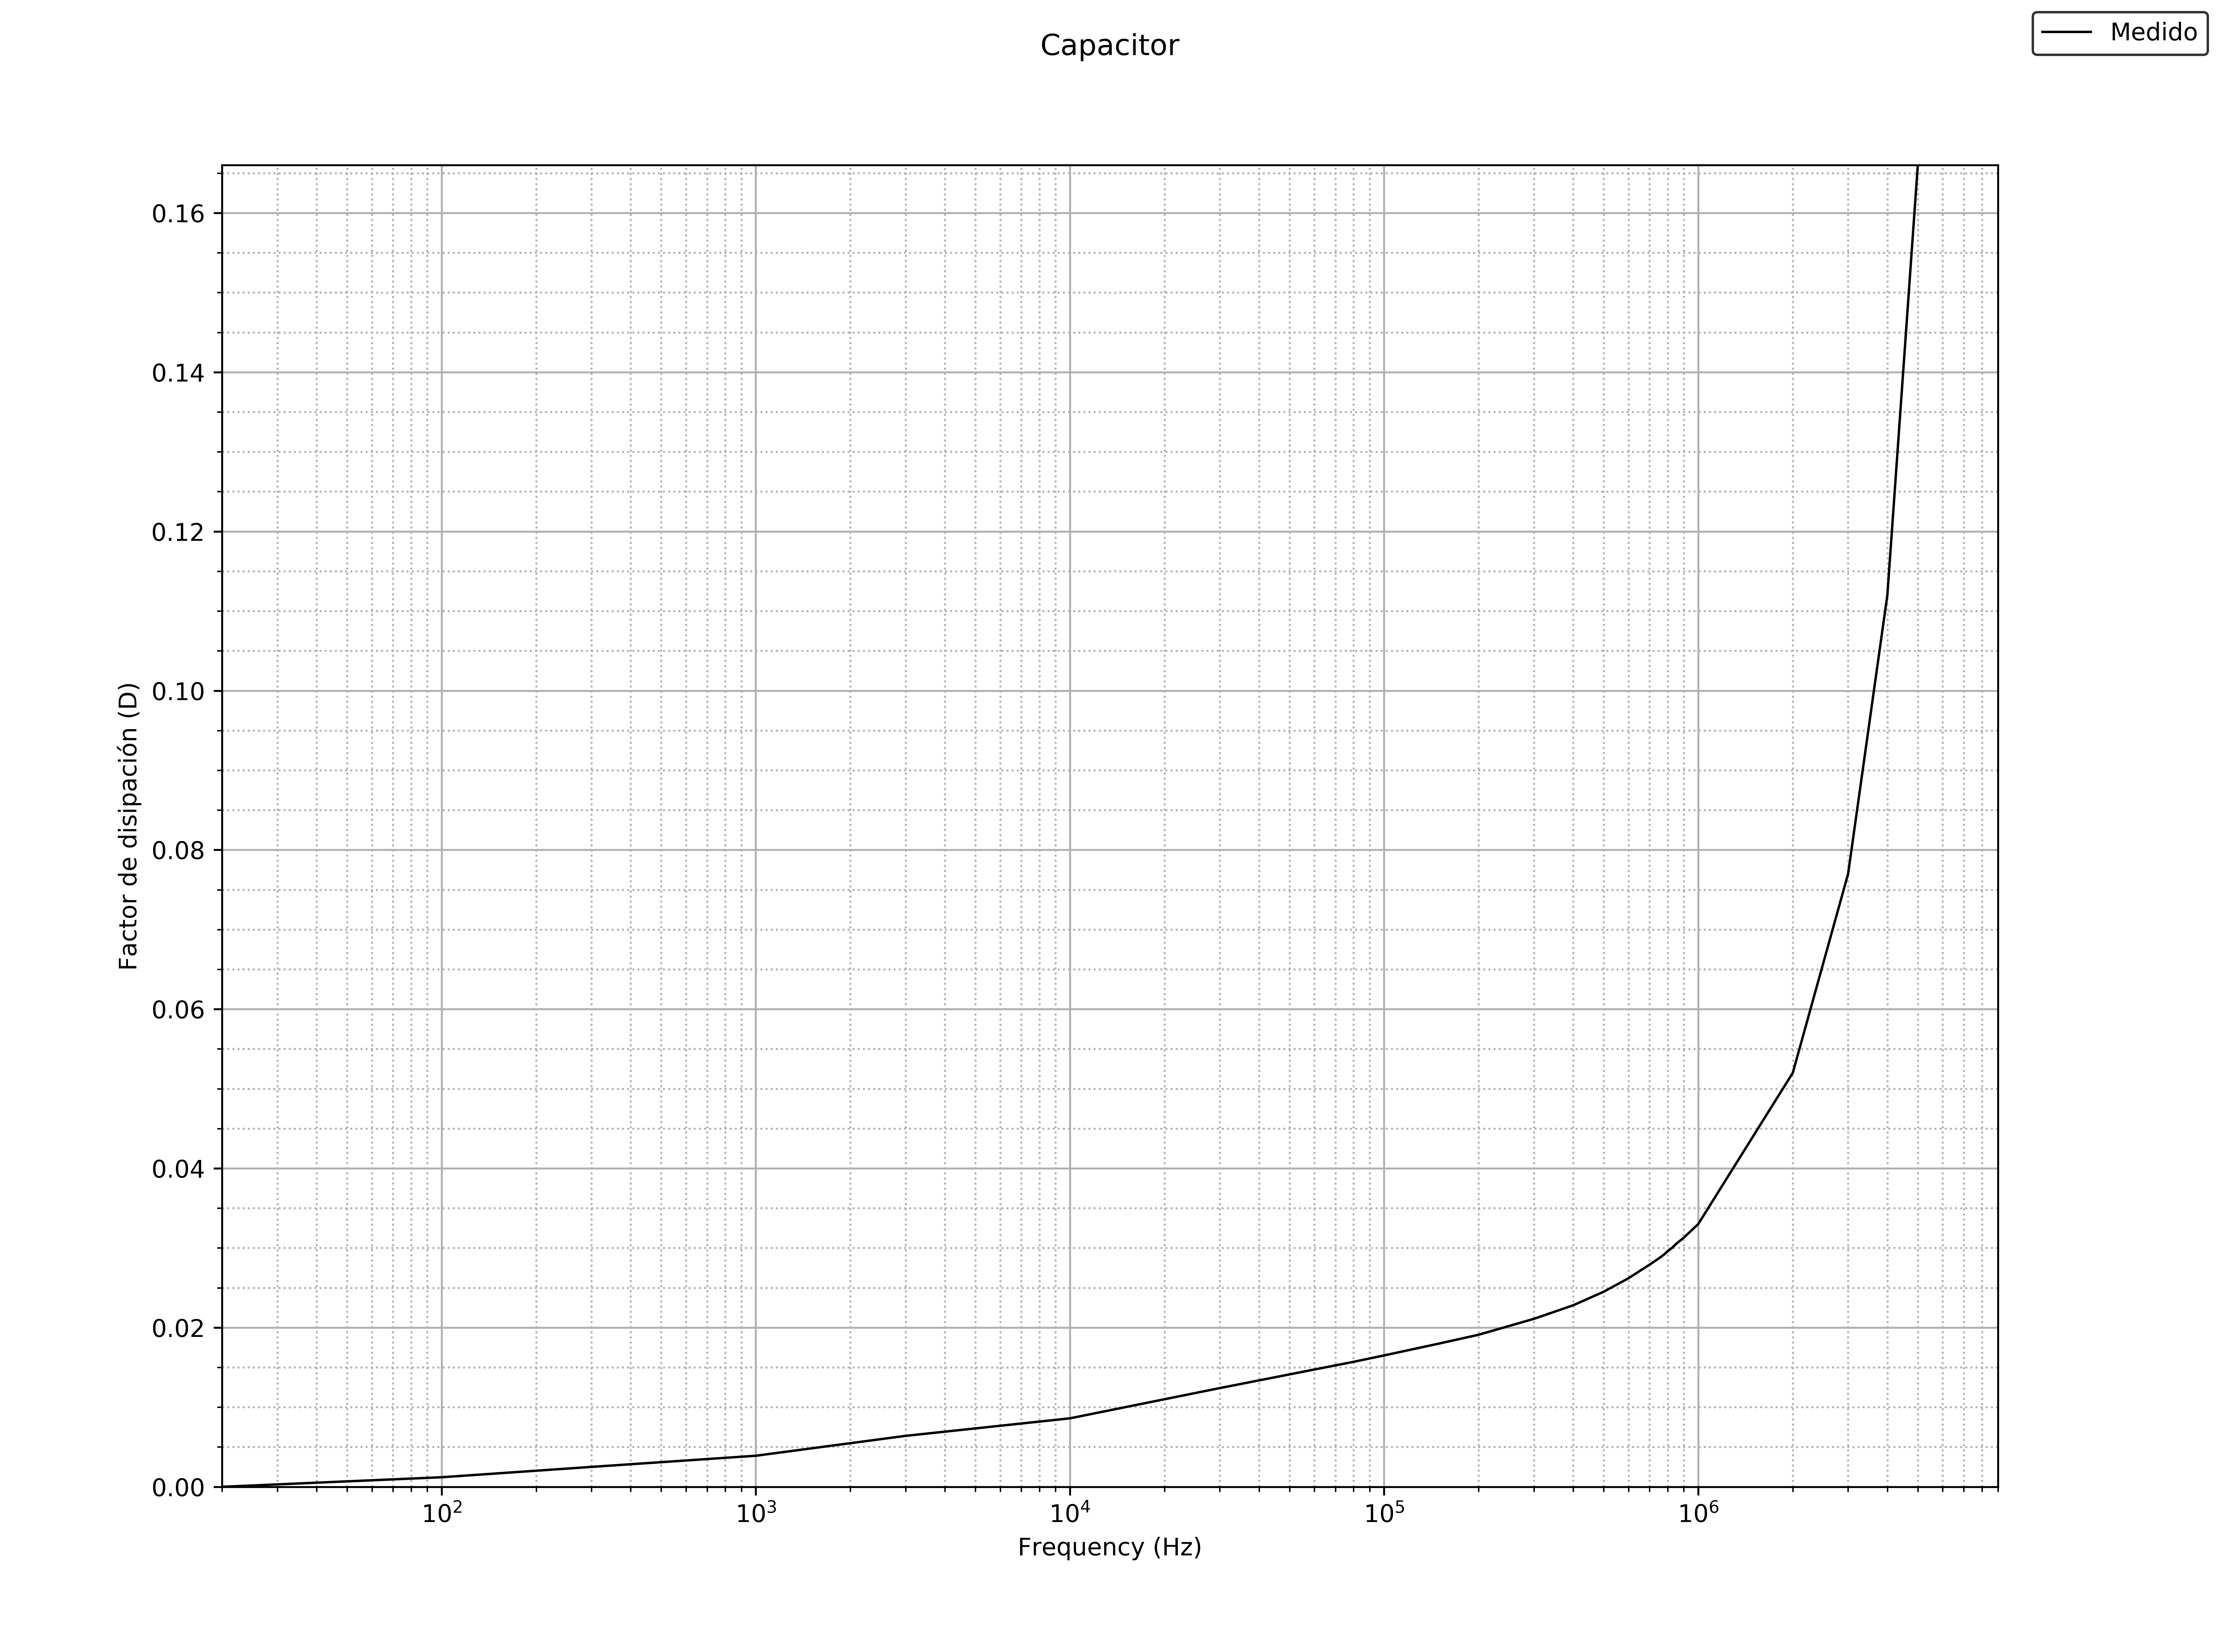
\includegraphics{Recursos/perdidas_medida_cap.png} \\
            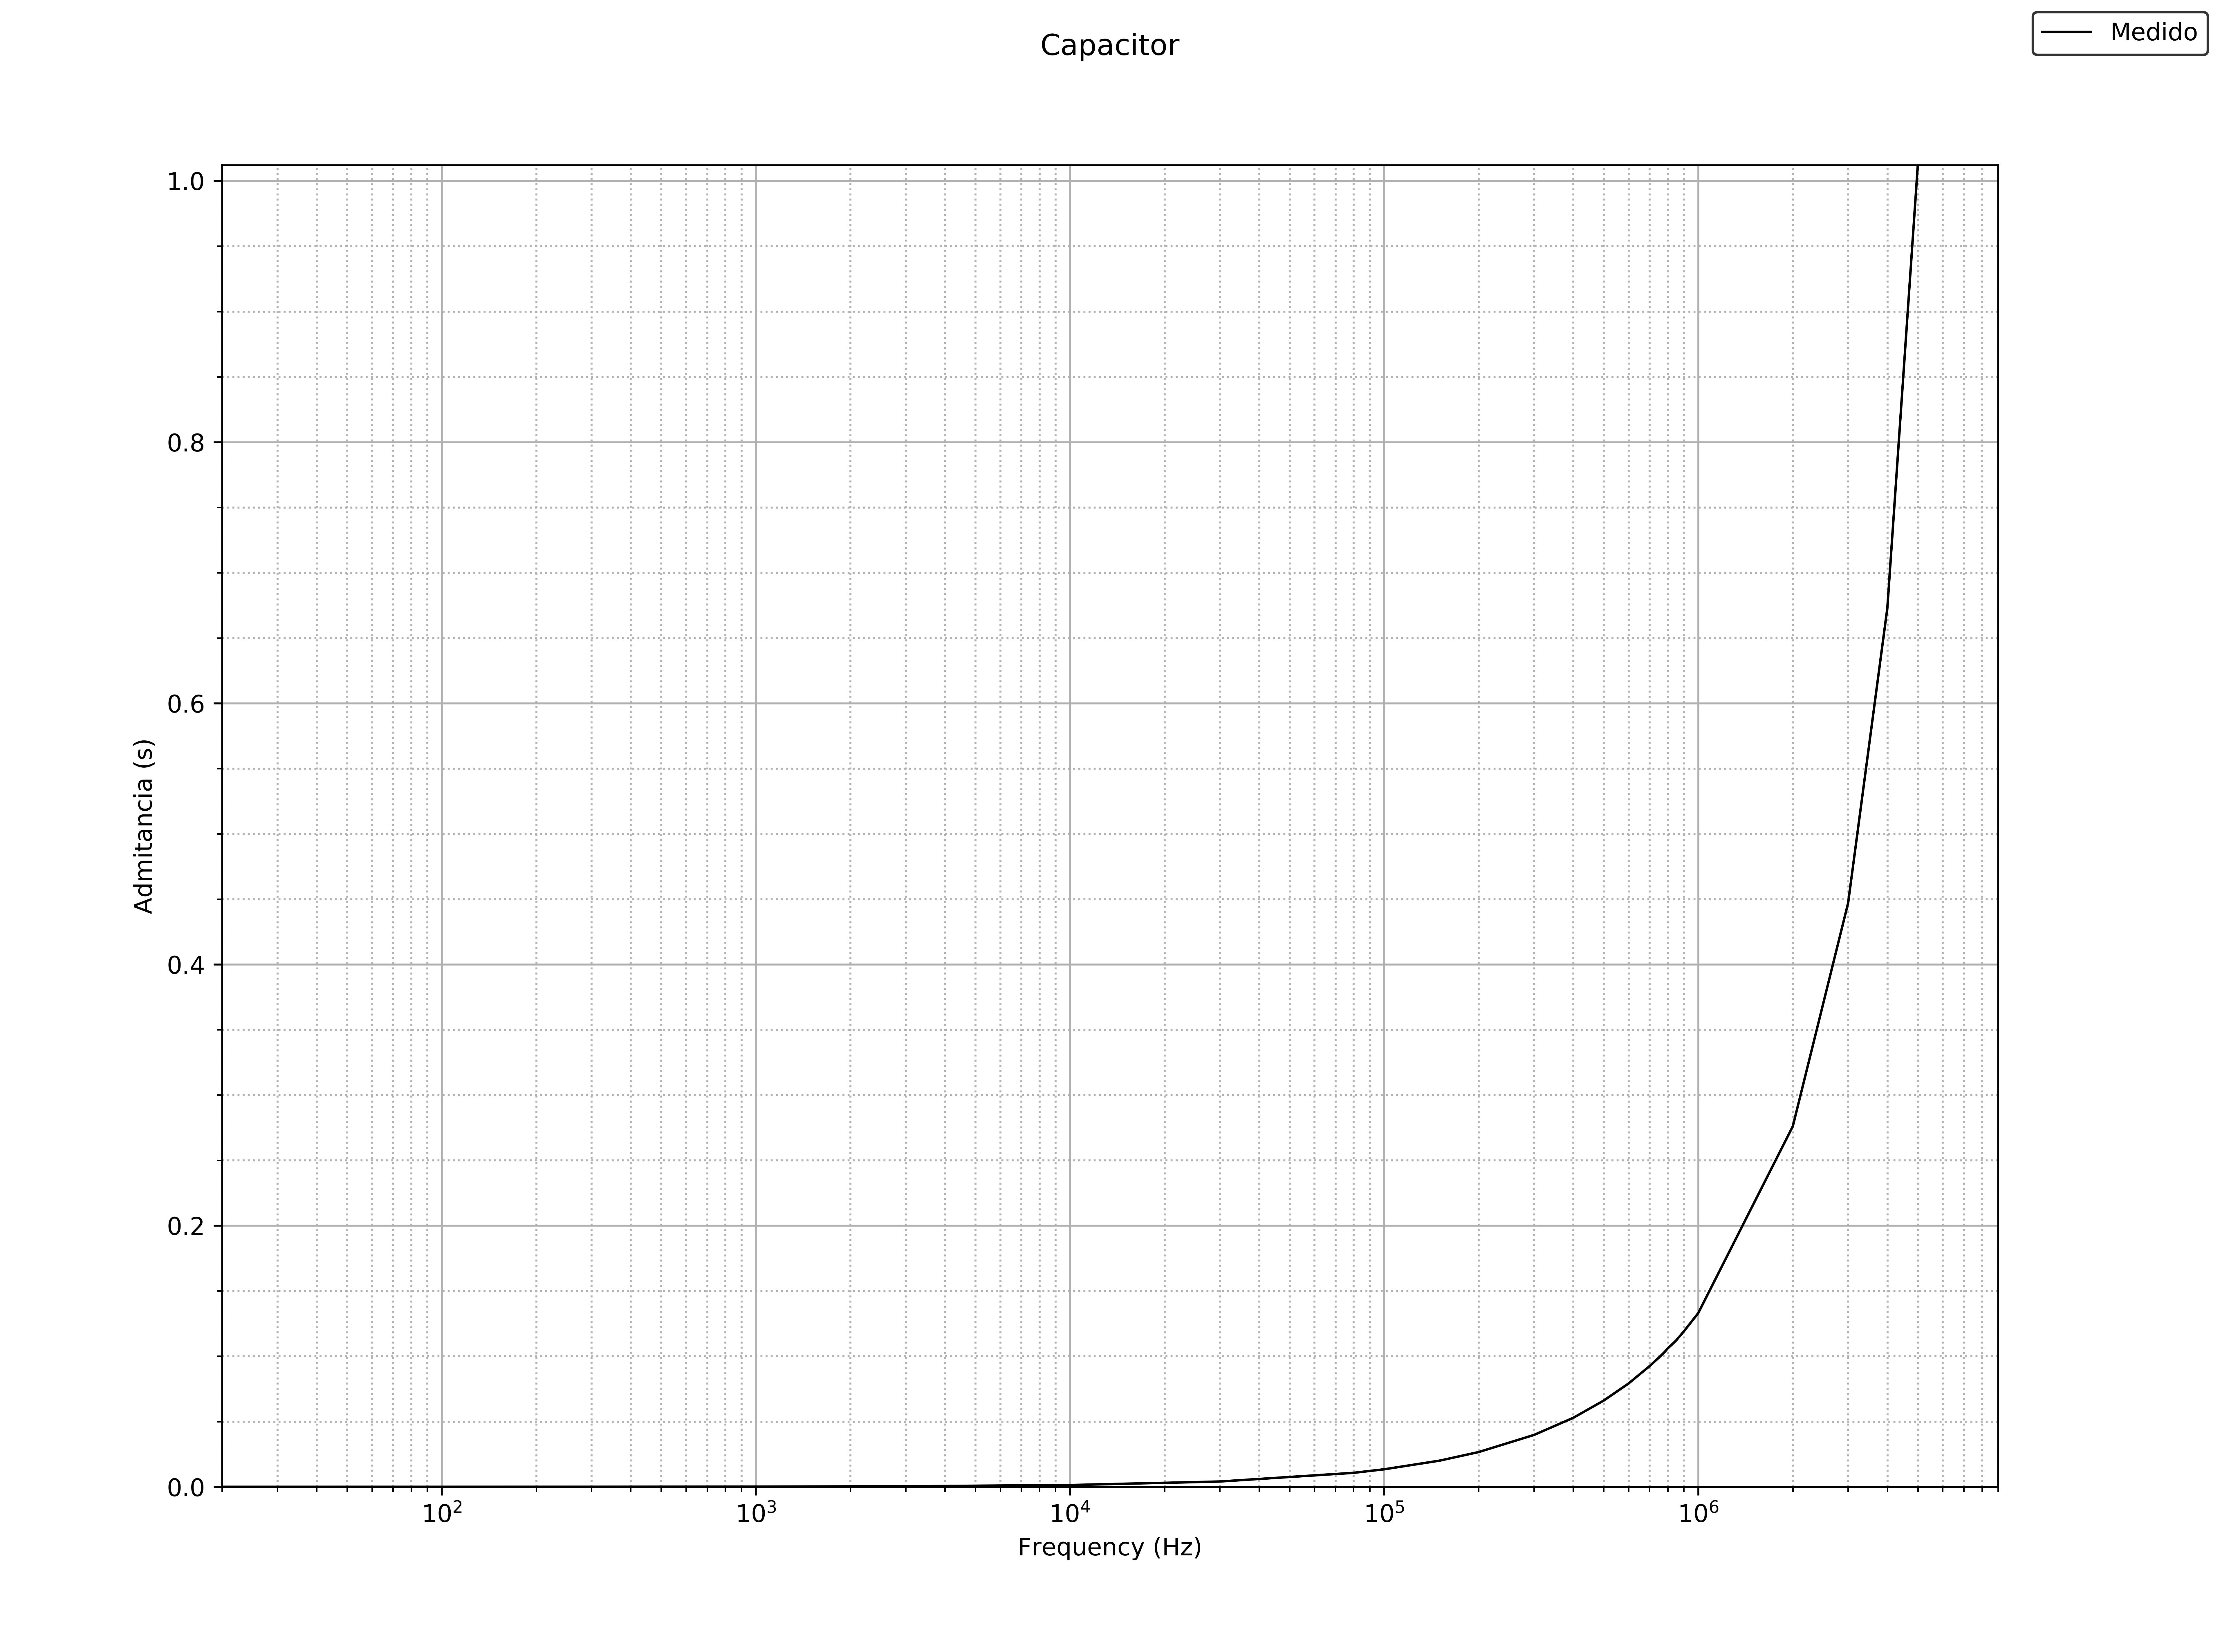
\includegraphics{Recursos/admitancia_medida_cap.png} &
            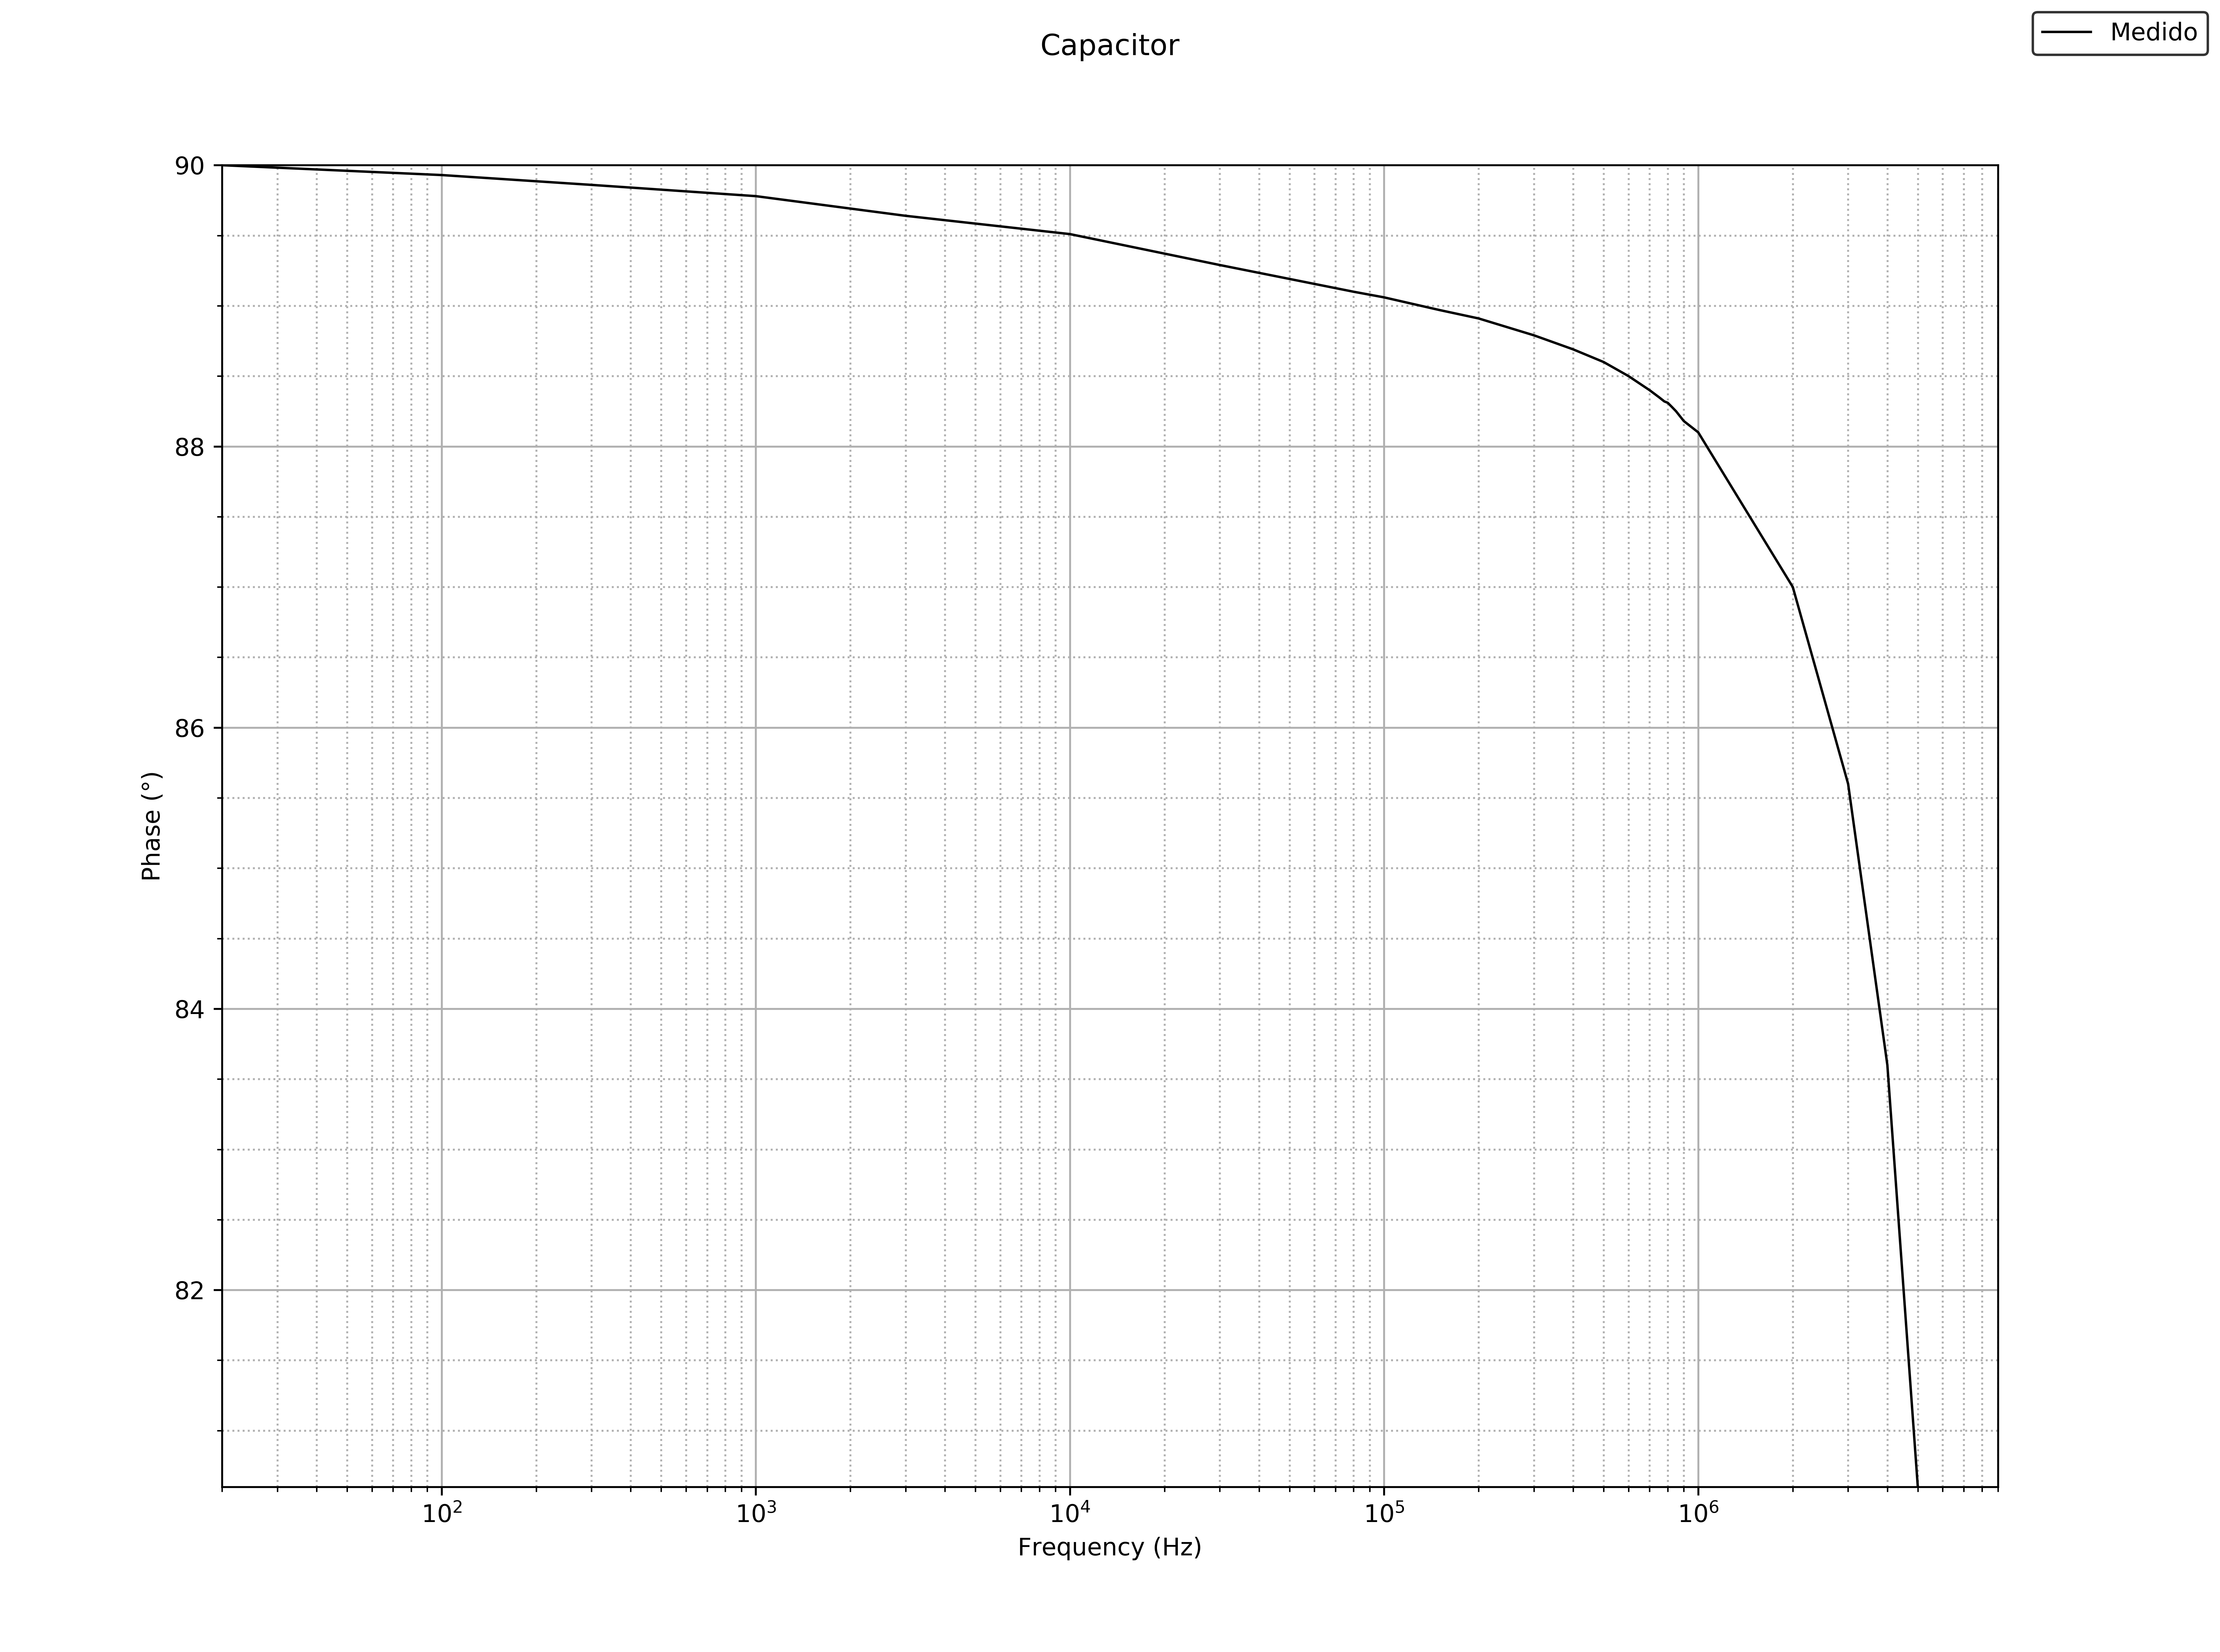
\includegraphics{Recursos/fase_medida_cap.png}

        \end{tabular}
    }
    \caption{Gr\'aficos realizados a partir de las mediciones}
    \label{fig:Med_CAP}
    
\end{figure}    


\subsubsection{Modelizaci\'on del comportamiento observado}
Se propone el circuito de la Figura \ref{fig:modelo_CAP} con el fin de encontrar un modelo que se ajuste al comportamiento real del capacitor tanto en impedancia como en fase.
\begin{figure}[H]
    \centering
    \resizebox{0.5\textwidth}{!}{
        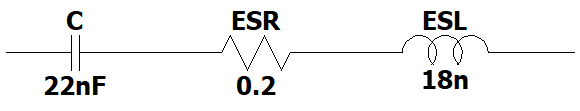
\includegraphics{Recursos/Modelo_cap.png}
    }
    \caption{Modelo de comportamiento del capacitor}
    \label{fig:modelo_CAP}
\end{figure}
El valor de la inductancia se parte de que la frecuencia de corte del sistema se encuentra en el punto donde el valor de capacidad arrojado por el analizador de impedancias pase de ser positivo a negativo, es decir, cuando el capacitor comienza a comportarse como un inductor. Del las mediciones se obtiene $f_{0} = 8MHz$. Luego, utilizando las f\'ormulas conocidas para un RLC serie mostradas en \ref{eq:RLC_CAP} y asumiendo que el valor de C es el nominal del componente utilizado.
\begin{equation}
    \omega_0 = \frac{1}{\sqrt{L \cdot C}} = 2 \cdot \pi \cdot f_0
    \label{eq:RLC_CAP}
\end{equation}
Resolviendo \ref{eq:RLC_CAP} se obtiene $L = 18nHy$.
Para ESR, se busca un valor iterando repetidas veces, hasta obtener una curva que se aproxime a la medida para la admitancia del capacitor.

Se muestran en la Figura \ref{fig:Comp_CAP}, los resultados obtenidos a partir del modelo elegido.

\begin{figure}[H]
    \centering
    \resizebox{\textwidth}{!}{
        \begin{tabular}{c c}
            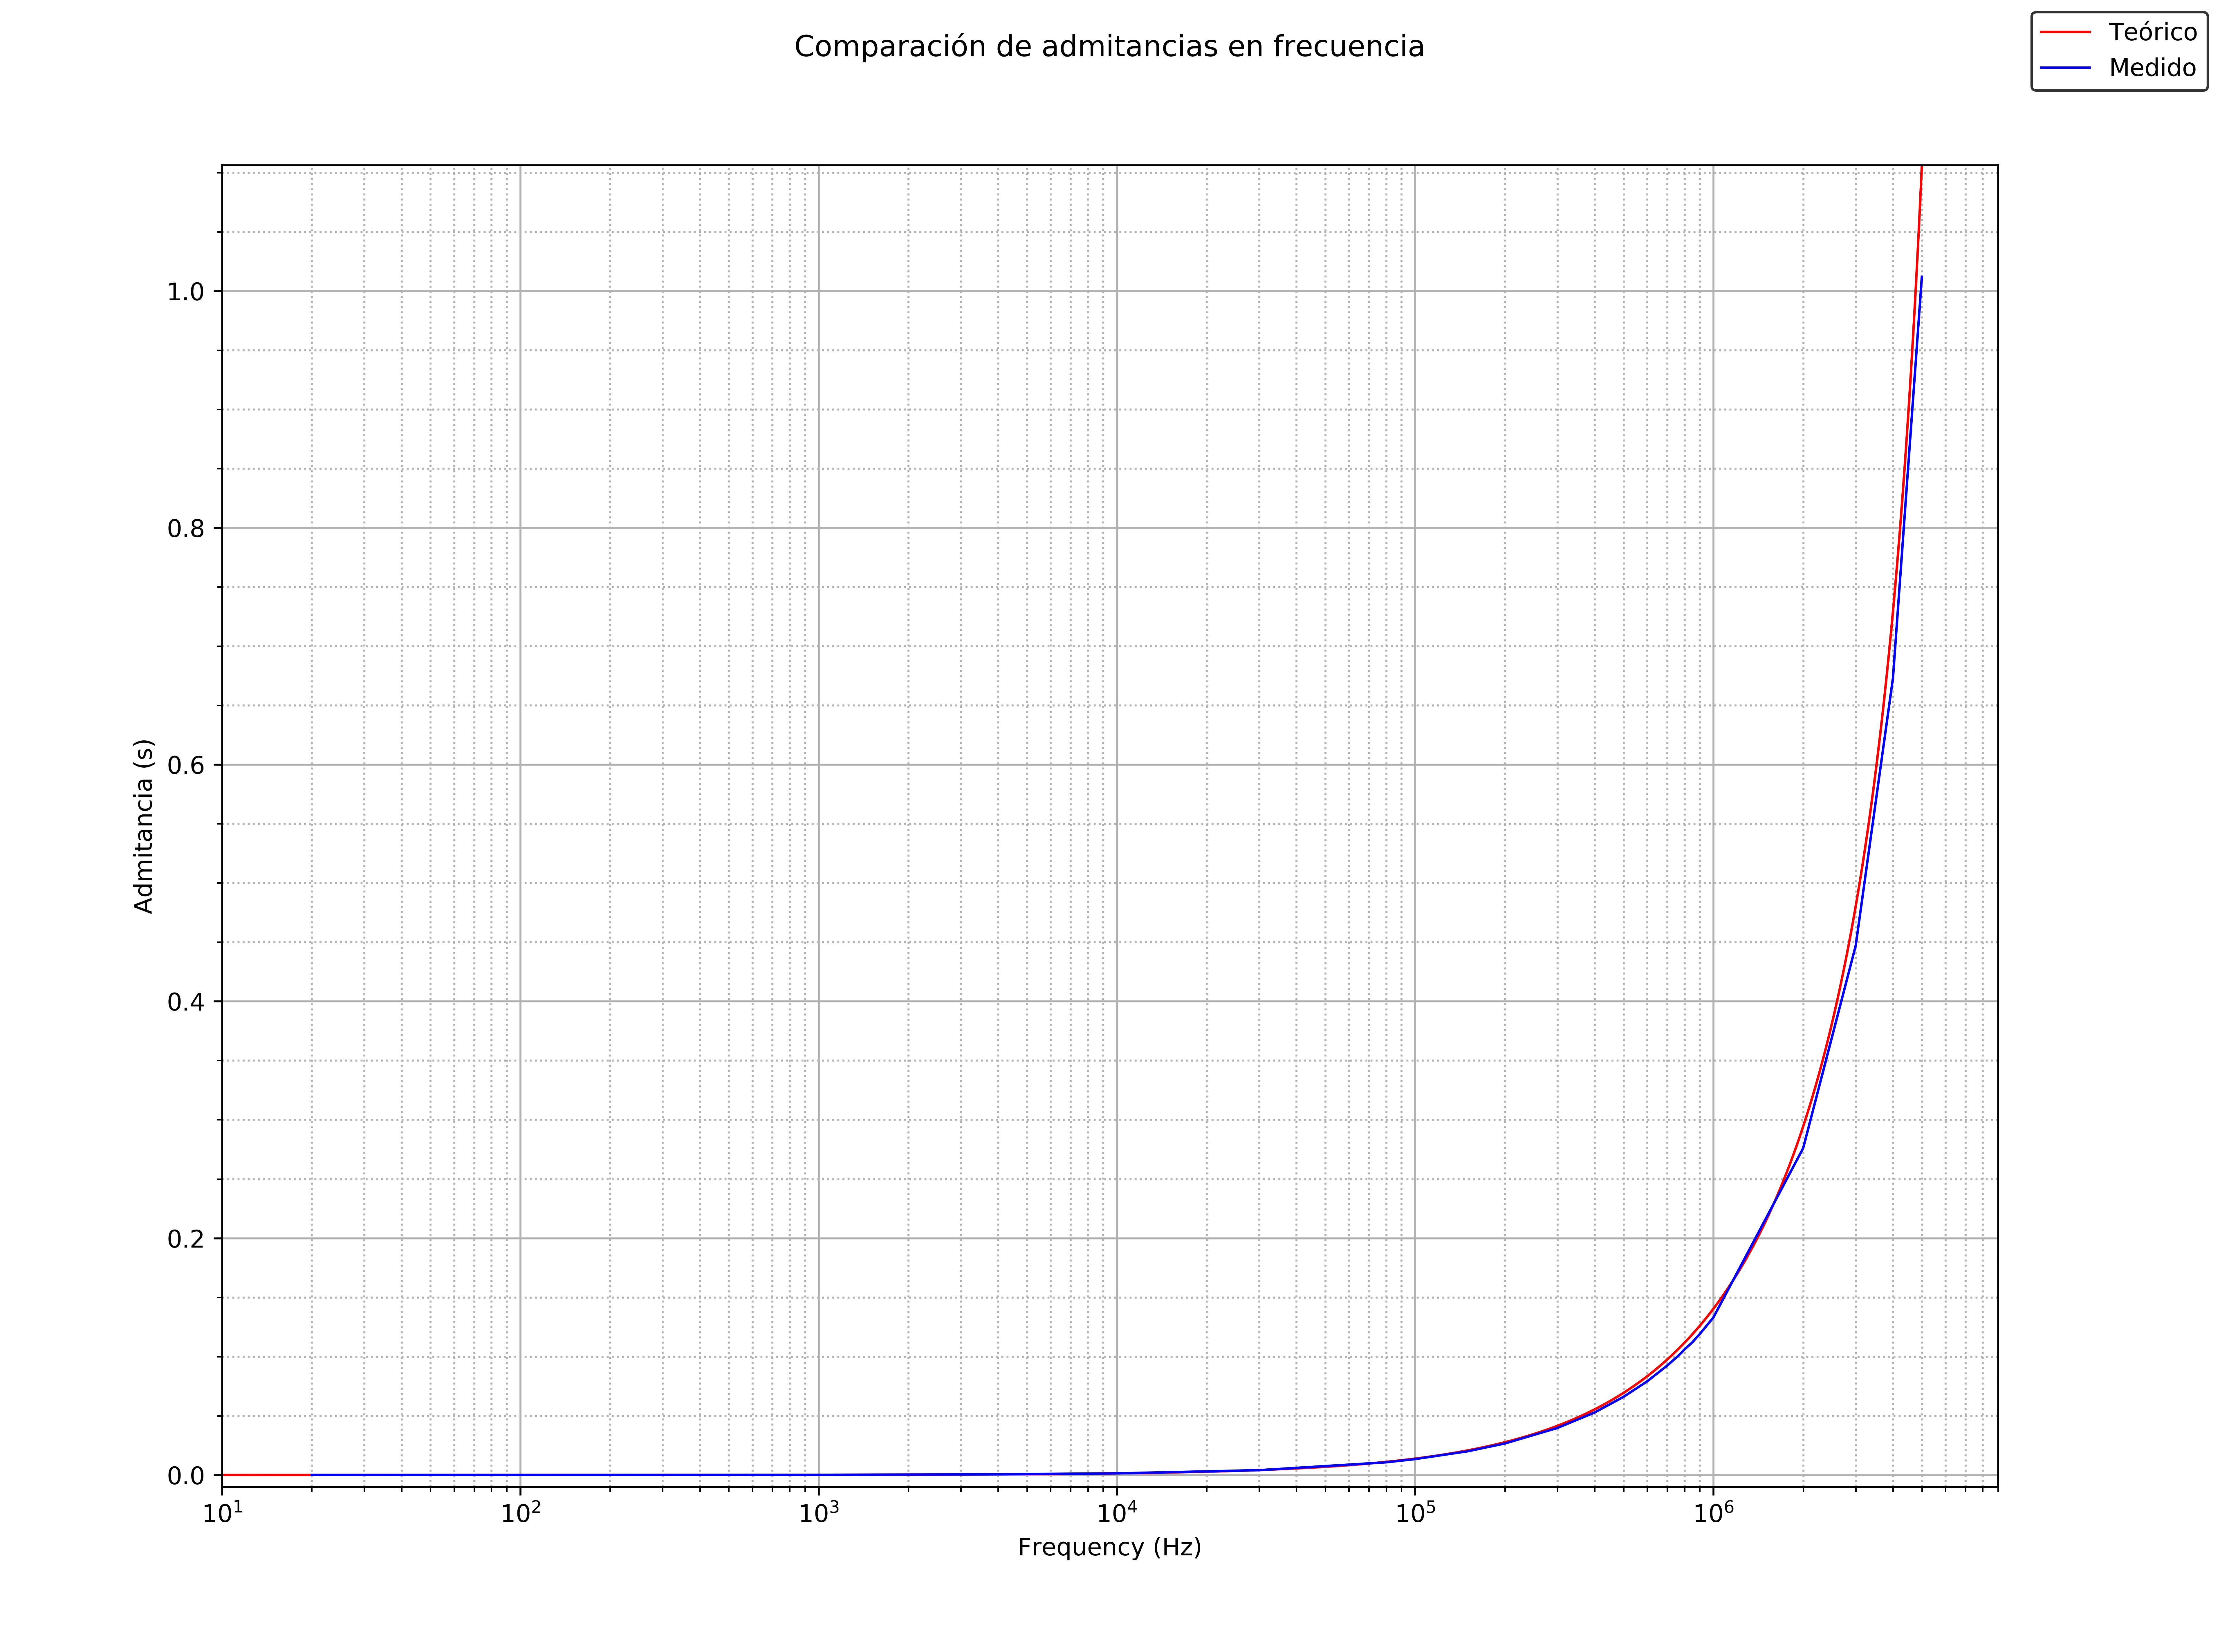
\includegraphics{Recursos/comp_admitancia_cap.png} &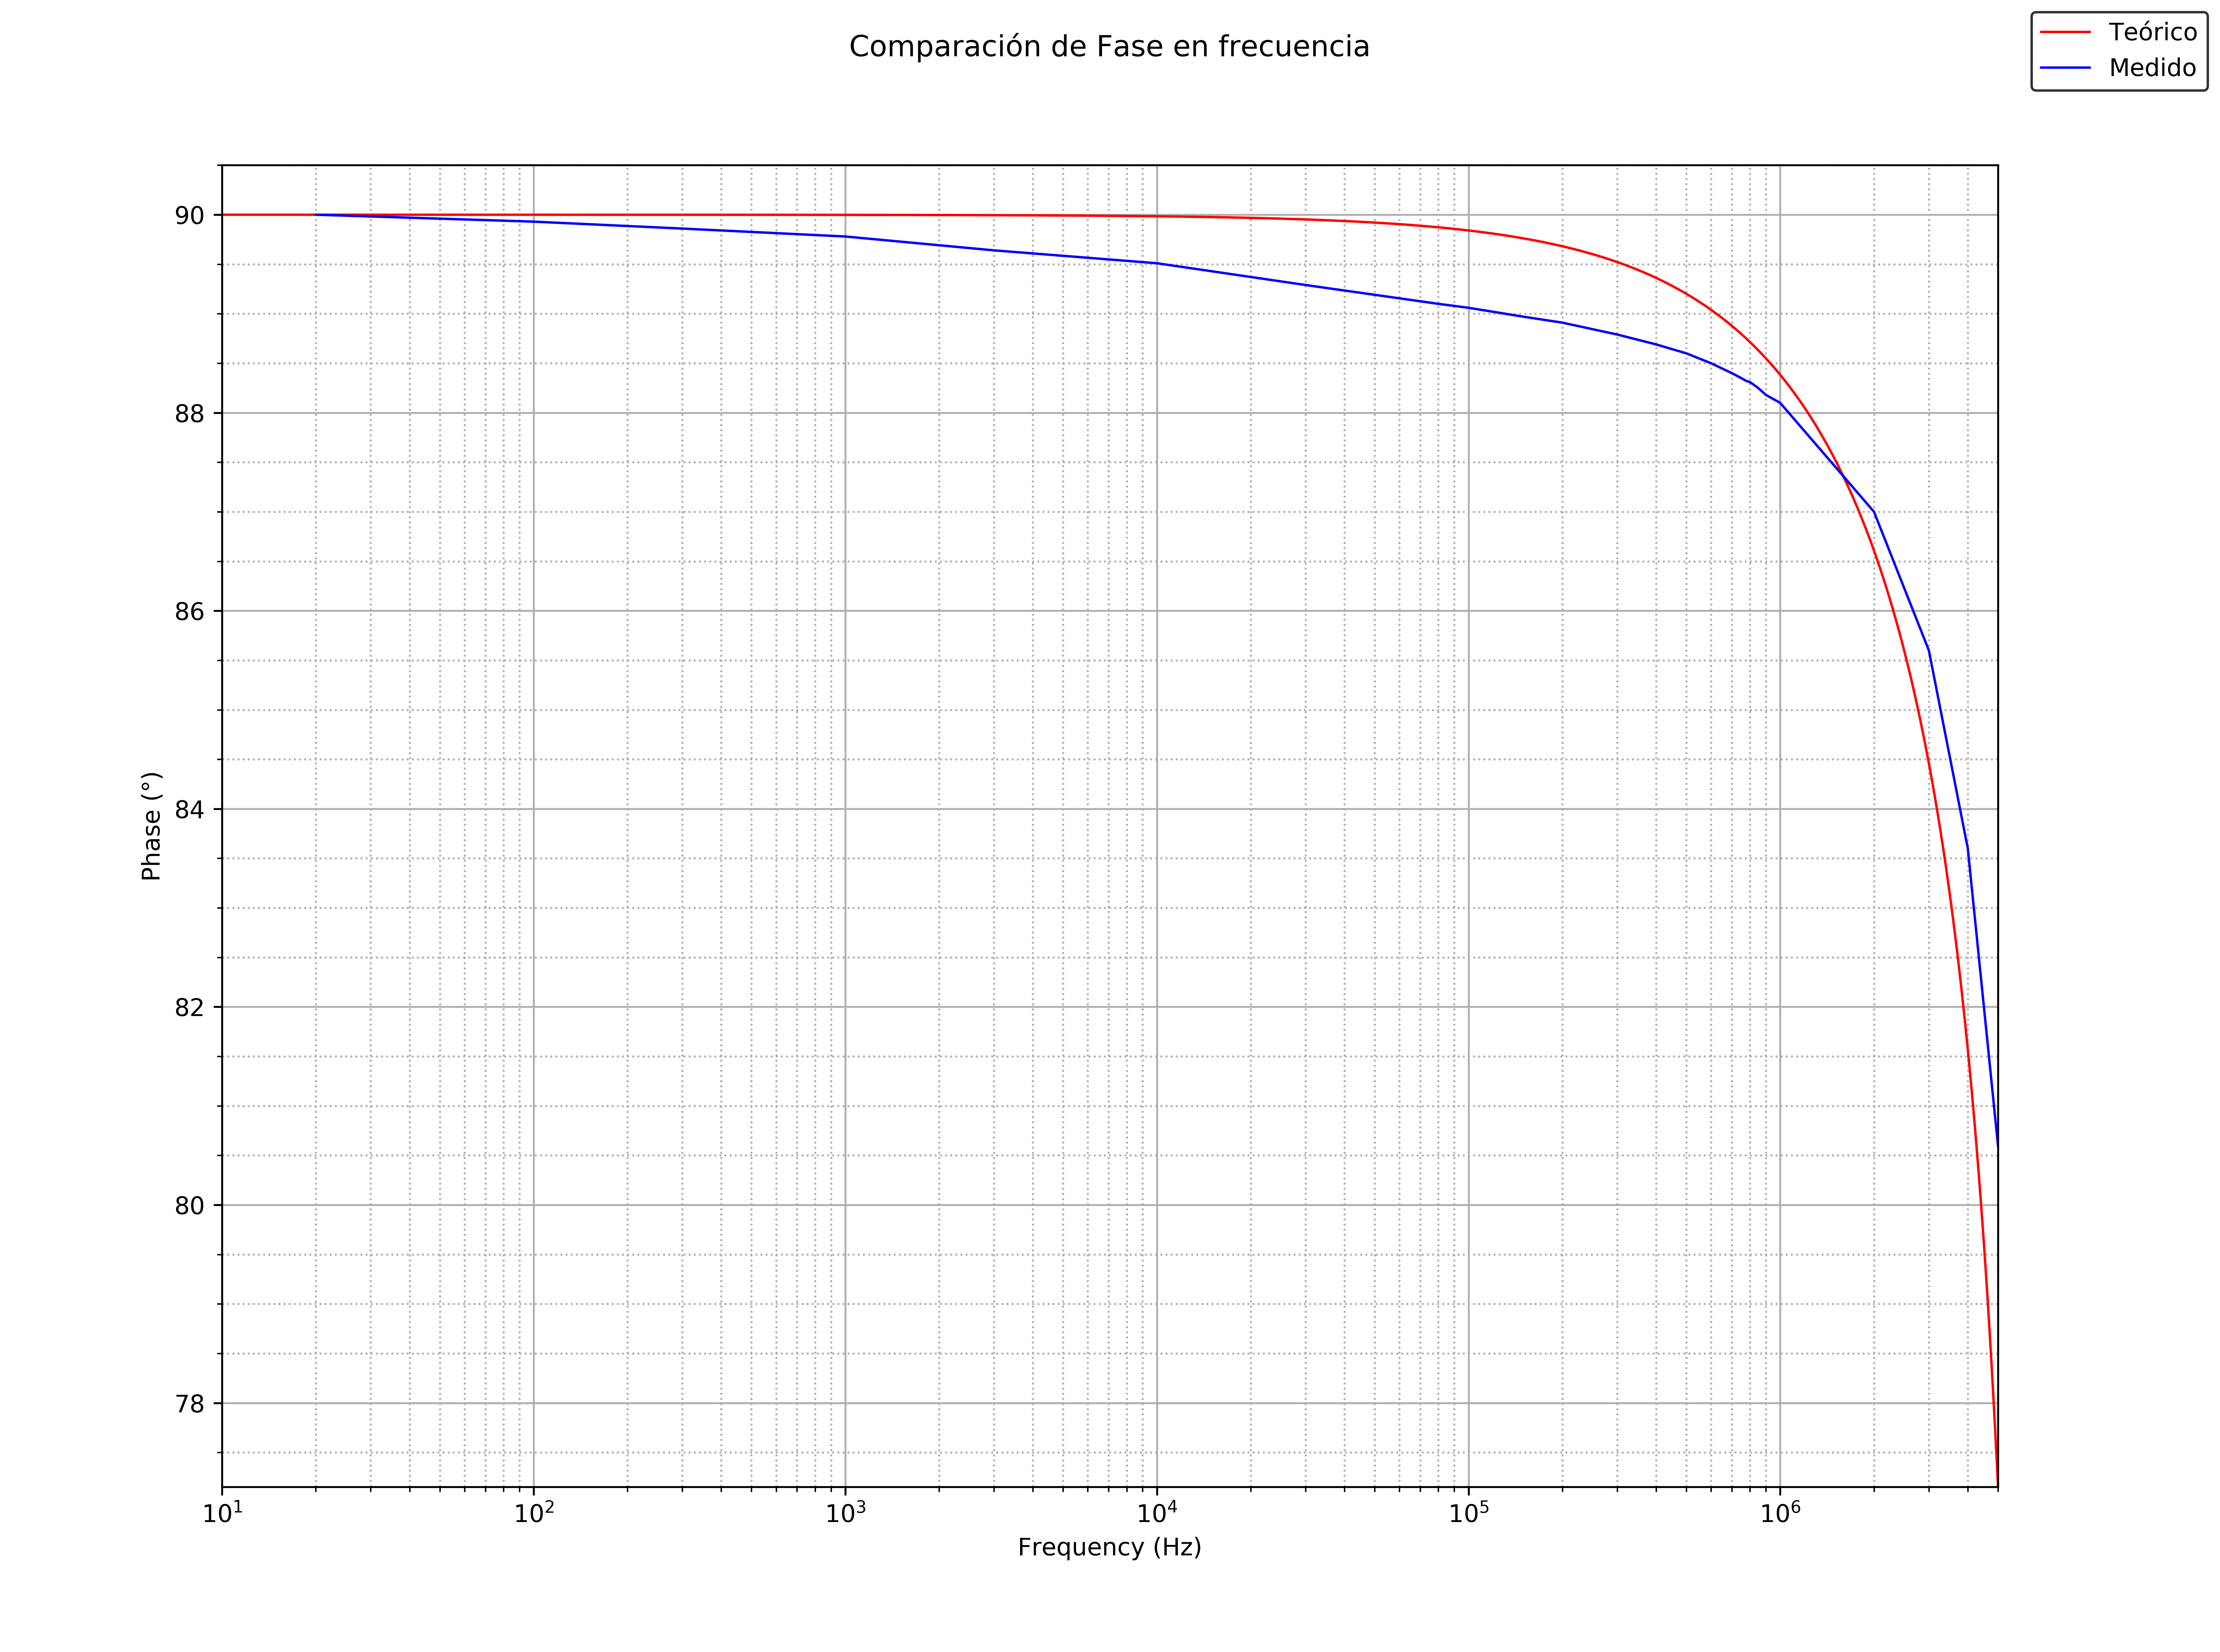
\includegraphics{Recursos/comp_fase_cap.png}
        \end{tabular}
        
    }
    \caption{Comparaci\'on entre mediciones y modelo de admitancia y fase en funci\'on de la frecuencia. }
        \label{fig:Comp_CAP}    
\end{figure}
Se observa un ajuste correcto en la comparaci\'on del modelo con las mediciones en el caso de la admitancia, lo que se corresponde con lo esperado ya que se dise\~na el circuito con ese fin. 

Si bien el comportamiento de la fase no coincide exactamente con el modelo, se puede observar que la forma es correcta. Se asume que estas diferencias son causadas por fen\'omenos no analizados en el capacitor como por ejemplo la variaci\'on de los valores de ESR y ESL con la frecuencia.

\subsection{Medici\'on del inductor}
Para la medici\'on se utiliza un inductor de $500\mu H$ con n\'ucleo de ferrite y se configura el analizador de impedancias en modelo serie para medir fase e impedancia. 
\subsubsection{Resultados}
Se muestran en la Tabla \ref{tab:Med_IND}  los resultados obtenidos de las mediciones y en la Figura \ref{fig:Med_IND} los respectivos  gr\'aficos realizados a partir de estas.
\begin{table}[H]
    \centering
    \resizebox{0.5\textwidth}{!}{%
        \begin{tabular}{ccccc}
            \hline
            \begin{tabular}[c]{@{}c@{}}Frecuencia\\   (Hz)
            \end{tabular} & Inductancia (Hy) & \begin{tabular}[c]{@{}c@{}}Factor de\\   calidad (Q)\end{tabular} & \multicolumn{1}{l}{Impedancia ($\Omega$)} & Fase ($^\circ$) \\ \hline
            10 & 5.00E-04 & 0 & 0.1 & 18.2 \\
            20 & 4.90E-04 & 1 & 1.13E-01 & 33 \\
            100 & 4.96E-04 & 3 & 0.328 & 71.6 \\
            300 & 4.92E-04 & 8 & 9.35E-01 & 82.6 \\
            1000 & 4.94E-04 & 16 & 3.11 & 86.4 \\
            3000 & 4.89E-04 & 23.5 & 9.23E+00 & 87.54 \\
            10000 & 4.89E-04 & 25 & 30.77 & 87.67 \\
            30000 & 4.77E-04 & 22.5 & 9.02E+01 & 87.43 \\
            80000 & 4.64E-04 & 17 & 2.34E+02 & 86.6 \\
            100000 & 4.66E-04 & 14.7 & 293 & 86.09 \\
            150000 & 4.66E-04 & 11.3 & 4.41E+02 & 84.93 \\
            200000 & 4.73E-04 & 8.9 & 5.98E+02 & 83.57 \\
            300000 & 5.00E-04 & 5.9 & 9.56E+02 & 80.47 \\
            400000 & 5.47E-04 & 4.1 & 1.41E+03 & 76.42 \\
            500000 & 6.20E-04 & 2.9 & 2.06E+03 & 70.7 \\
            600000 & 7.15E-04 & 1.8 & 3.07E+03 & 61.5 \\
            700000 & 7.52E-04 & 1 & 4.73E+03 & 44.4 \\
            750000 & 6.18E-04 & 0.6 & 5.80E+03 & 30.24 \\
            780000 & 4.32E-04 & 0.4 & 6.37E+03 & 19.4 \\
            800000 & 2.56E-04 & 0.2 & 6.66E+03 & 11.11 \\
            825000 & 2.30E-05 & 0 & 6.84E+03 & 1.04 \\
            850000 & -2.05E-04 & 0.2 & 6.78E+03 & -9.29 \\
            875000 & -3.80E-04 & 0.3 & 6.54E+03 & -18.86 \\
            900000 & -5.03E-04 & 0.5 & 6.16E+03 & -27.5 \\
            950000 & -5.82E-04 & 0.9 & 5.31E+03 & -40.89 \\
            1000000 & -5.53E-04 & 1.2 & 4.48E+03 & -50.73 \\
            1250000 & -2.90E-04 & 2.8 & 2.47E+03 & -70.5 \\
            1500000 & -1.70E-04 & 4.4 & 1.71E+03 & -77.11 \\
            1650000 & -1.38E-04 & 5.3 & 1.46E+03 & -79.25 \\
            1750000 & -1.19E-04 & 5.8 & 1.33E+03 & -80.31 \\
            2000000 & -8.59E-05 & 7.3 & 1.08E+03 & -82.24 \\
            3000000 & -3.43E-05 & 12.8 & 6.48E+02 & -85.51 \\
            4000000 & -1.86E-05 & 17.5 & 4.66E+02 & -86.7 \\
            5000000 & -1.16E-05 & 21.2 & 3.65E+02 & -87.27 \\
            10000000 & -2.70E-06 & 24.6 & 170.4 & -87.64 \\ \hline
        \end{tabular}%
    }
    \caption{Mediciones del inductor}
    \label{tab:Med_IND}
\end{table}
\begin{figure}[H]
    \centering
    \resizebox{\textwidth}{!}{
        \begin{tabular}{c c}
            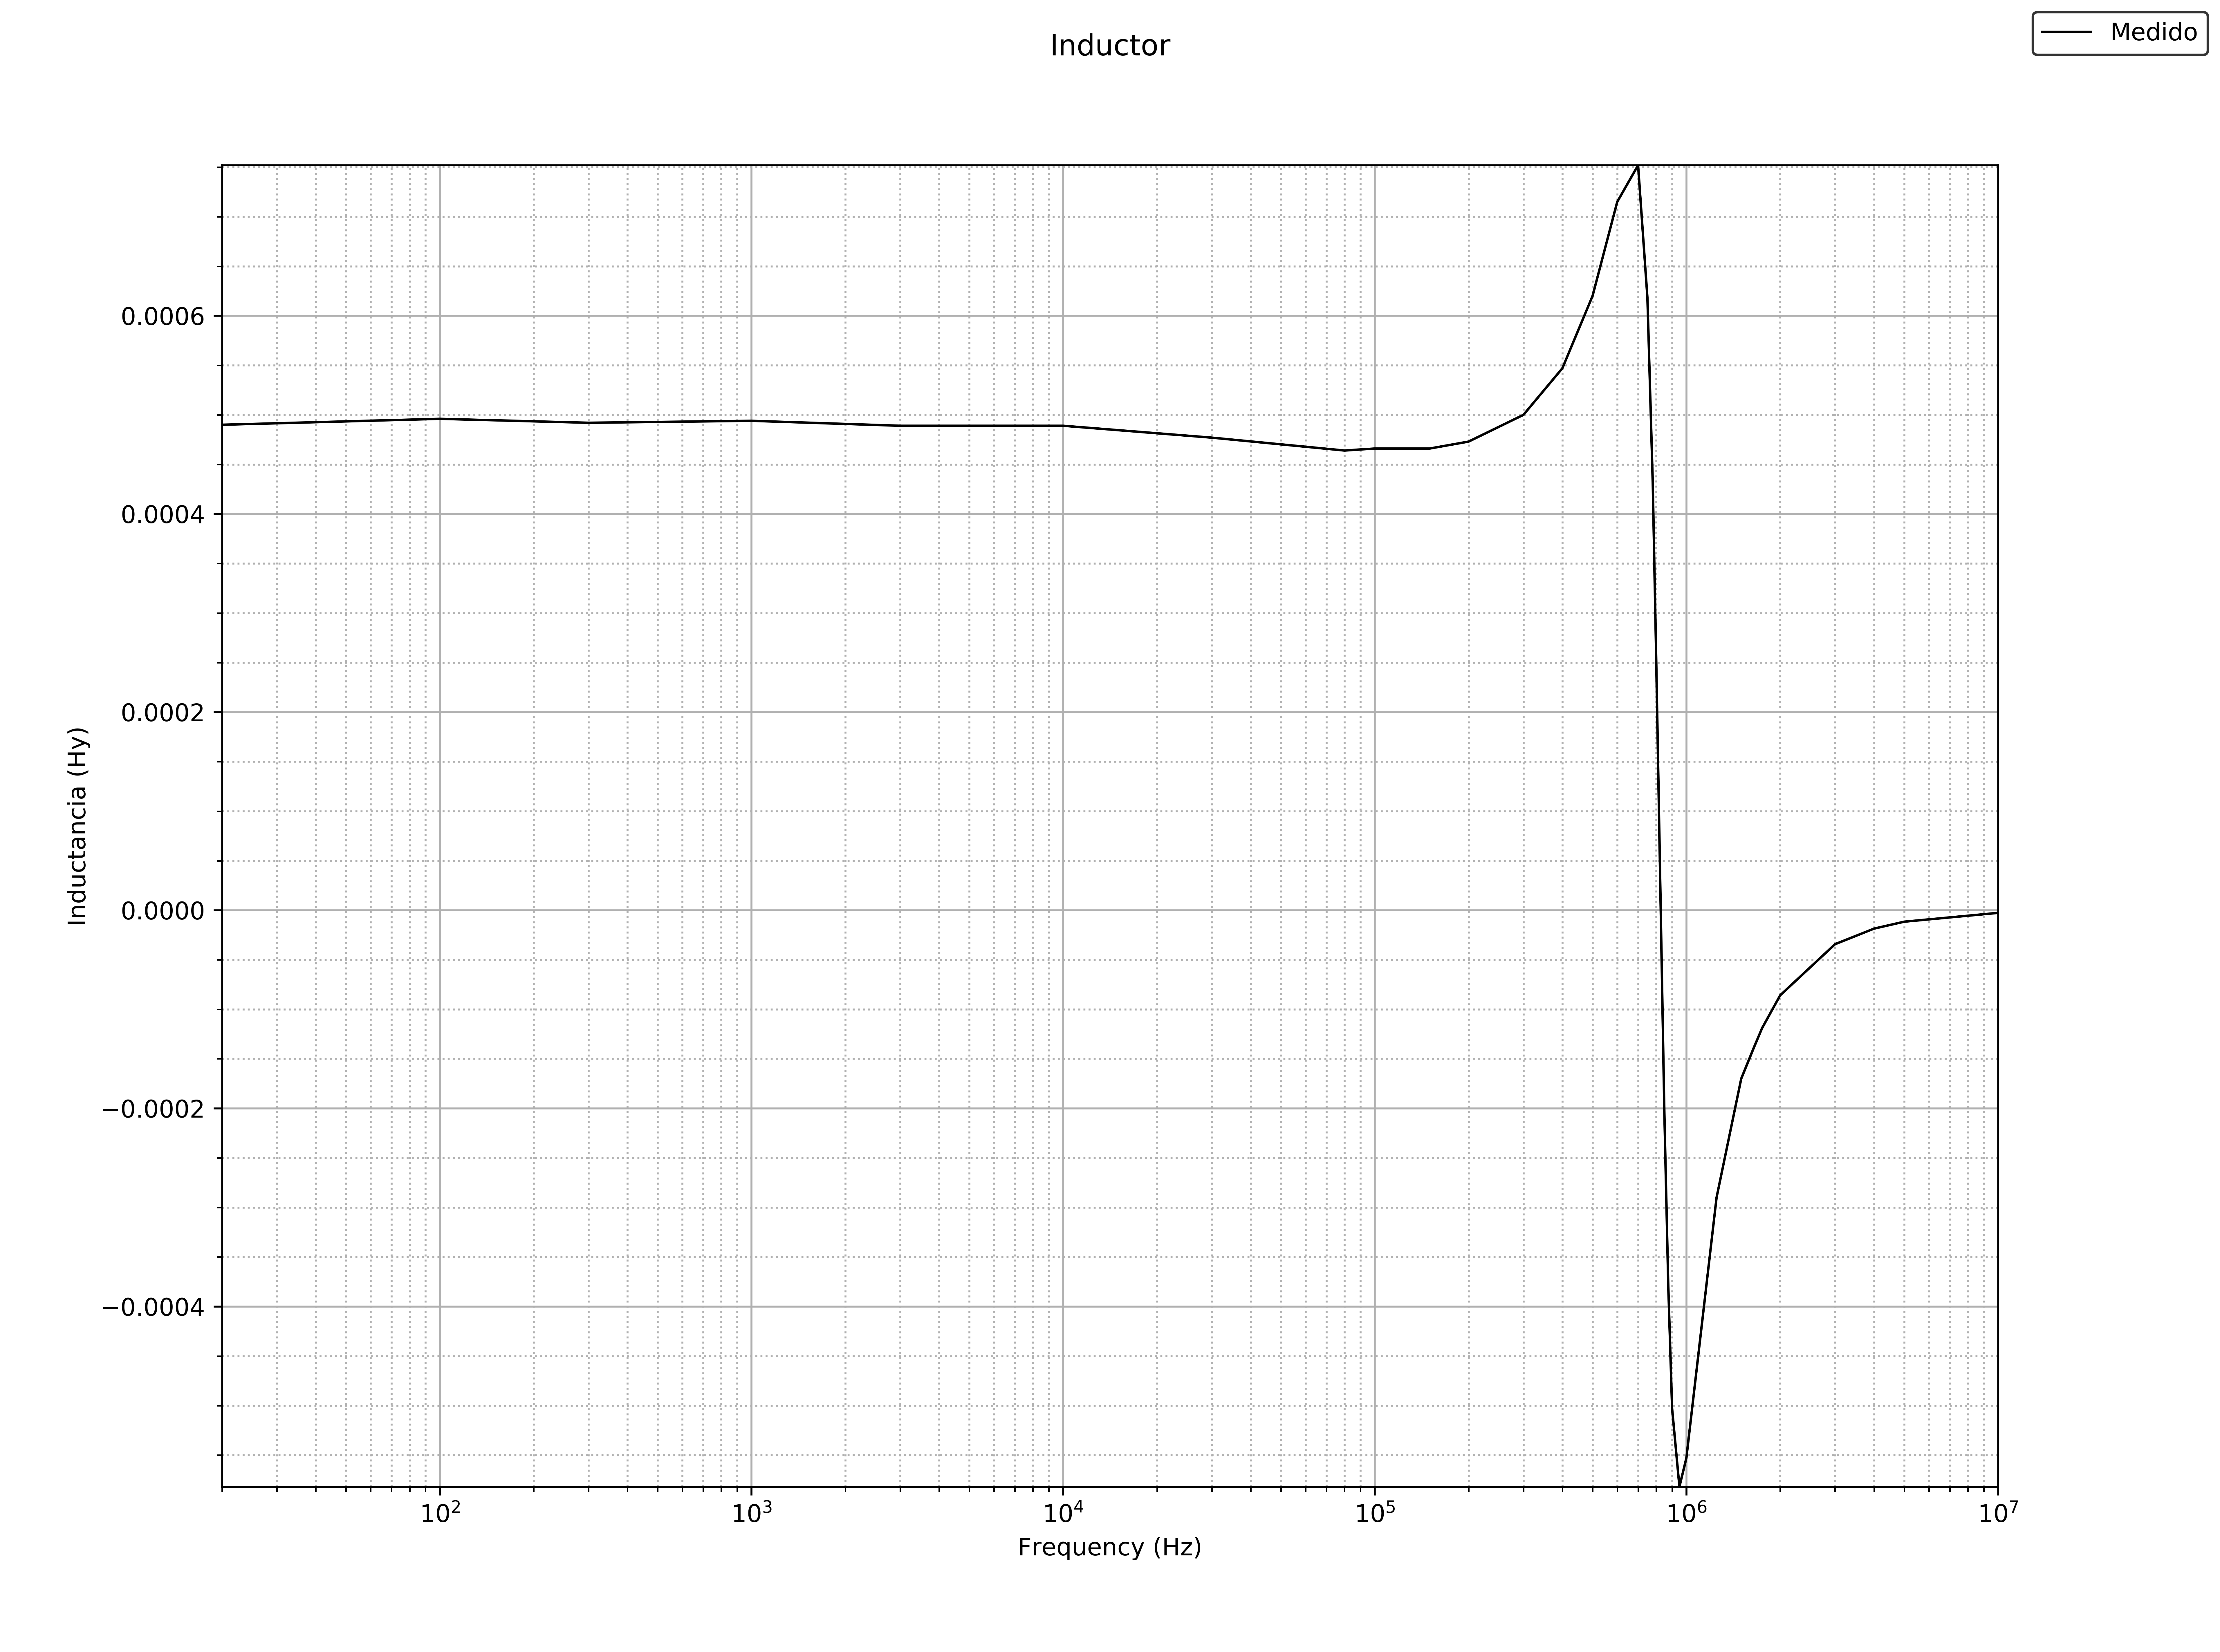
\includegraphics{Recursos/inductancia_medida_ind.png}&
            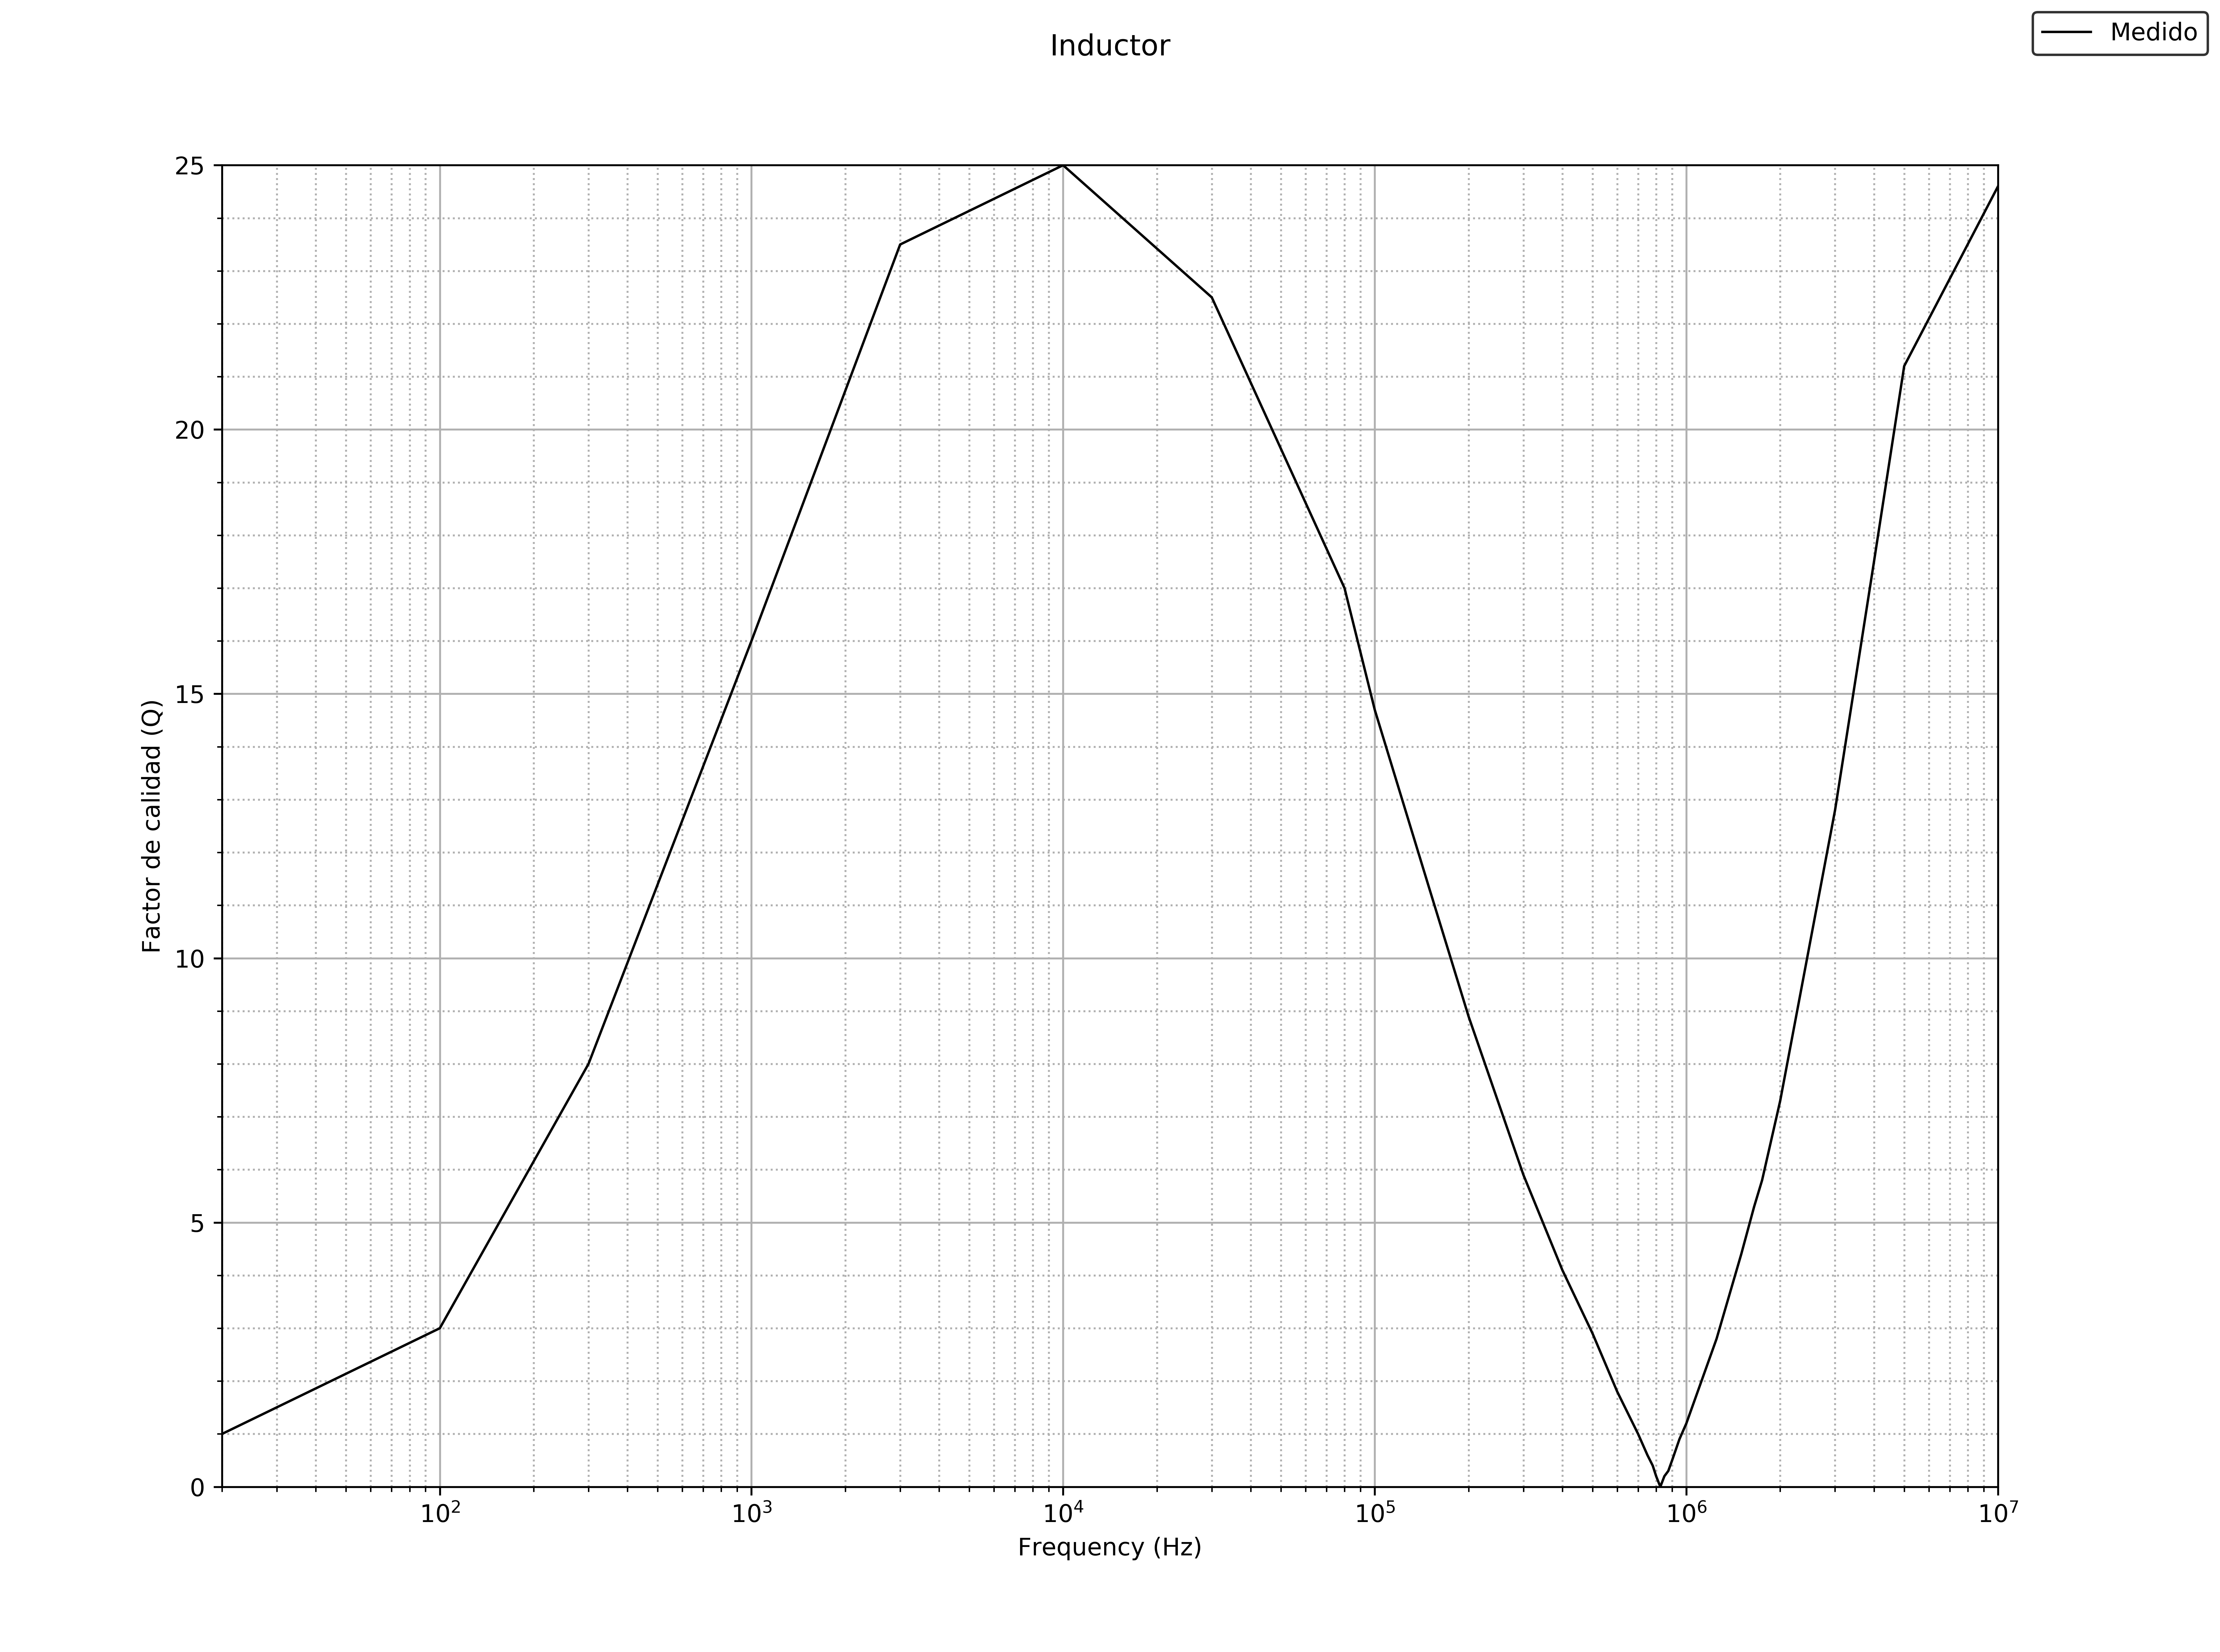
\includegraphics{Recursos/calidad_medida_ind.png} \\
            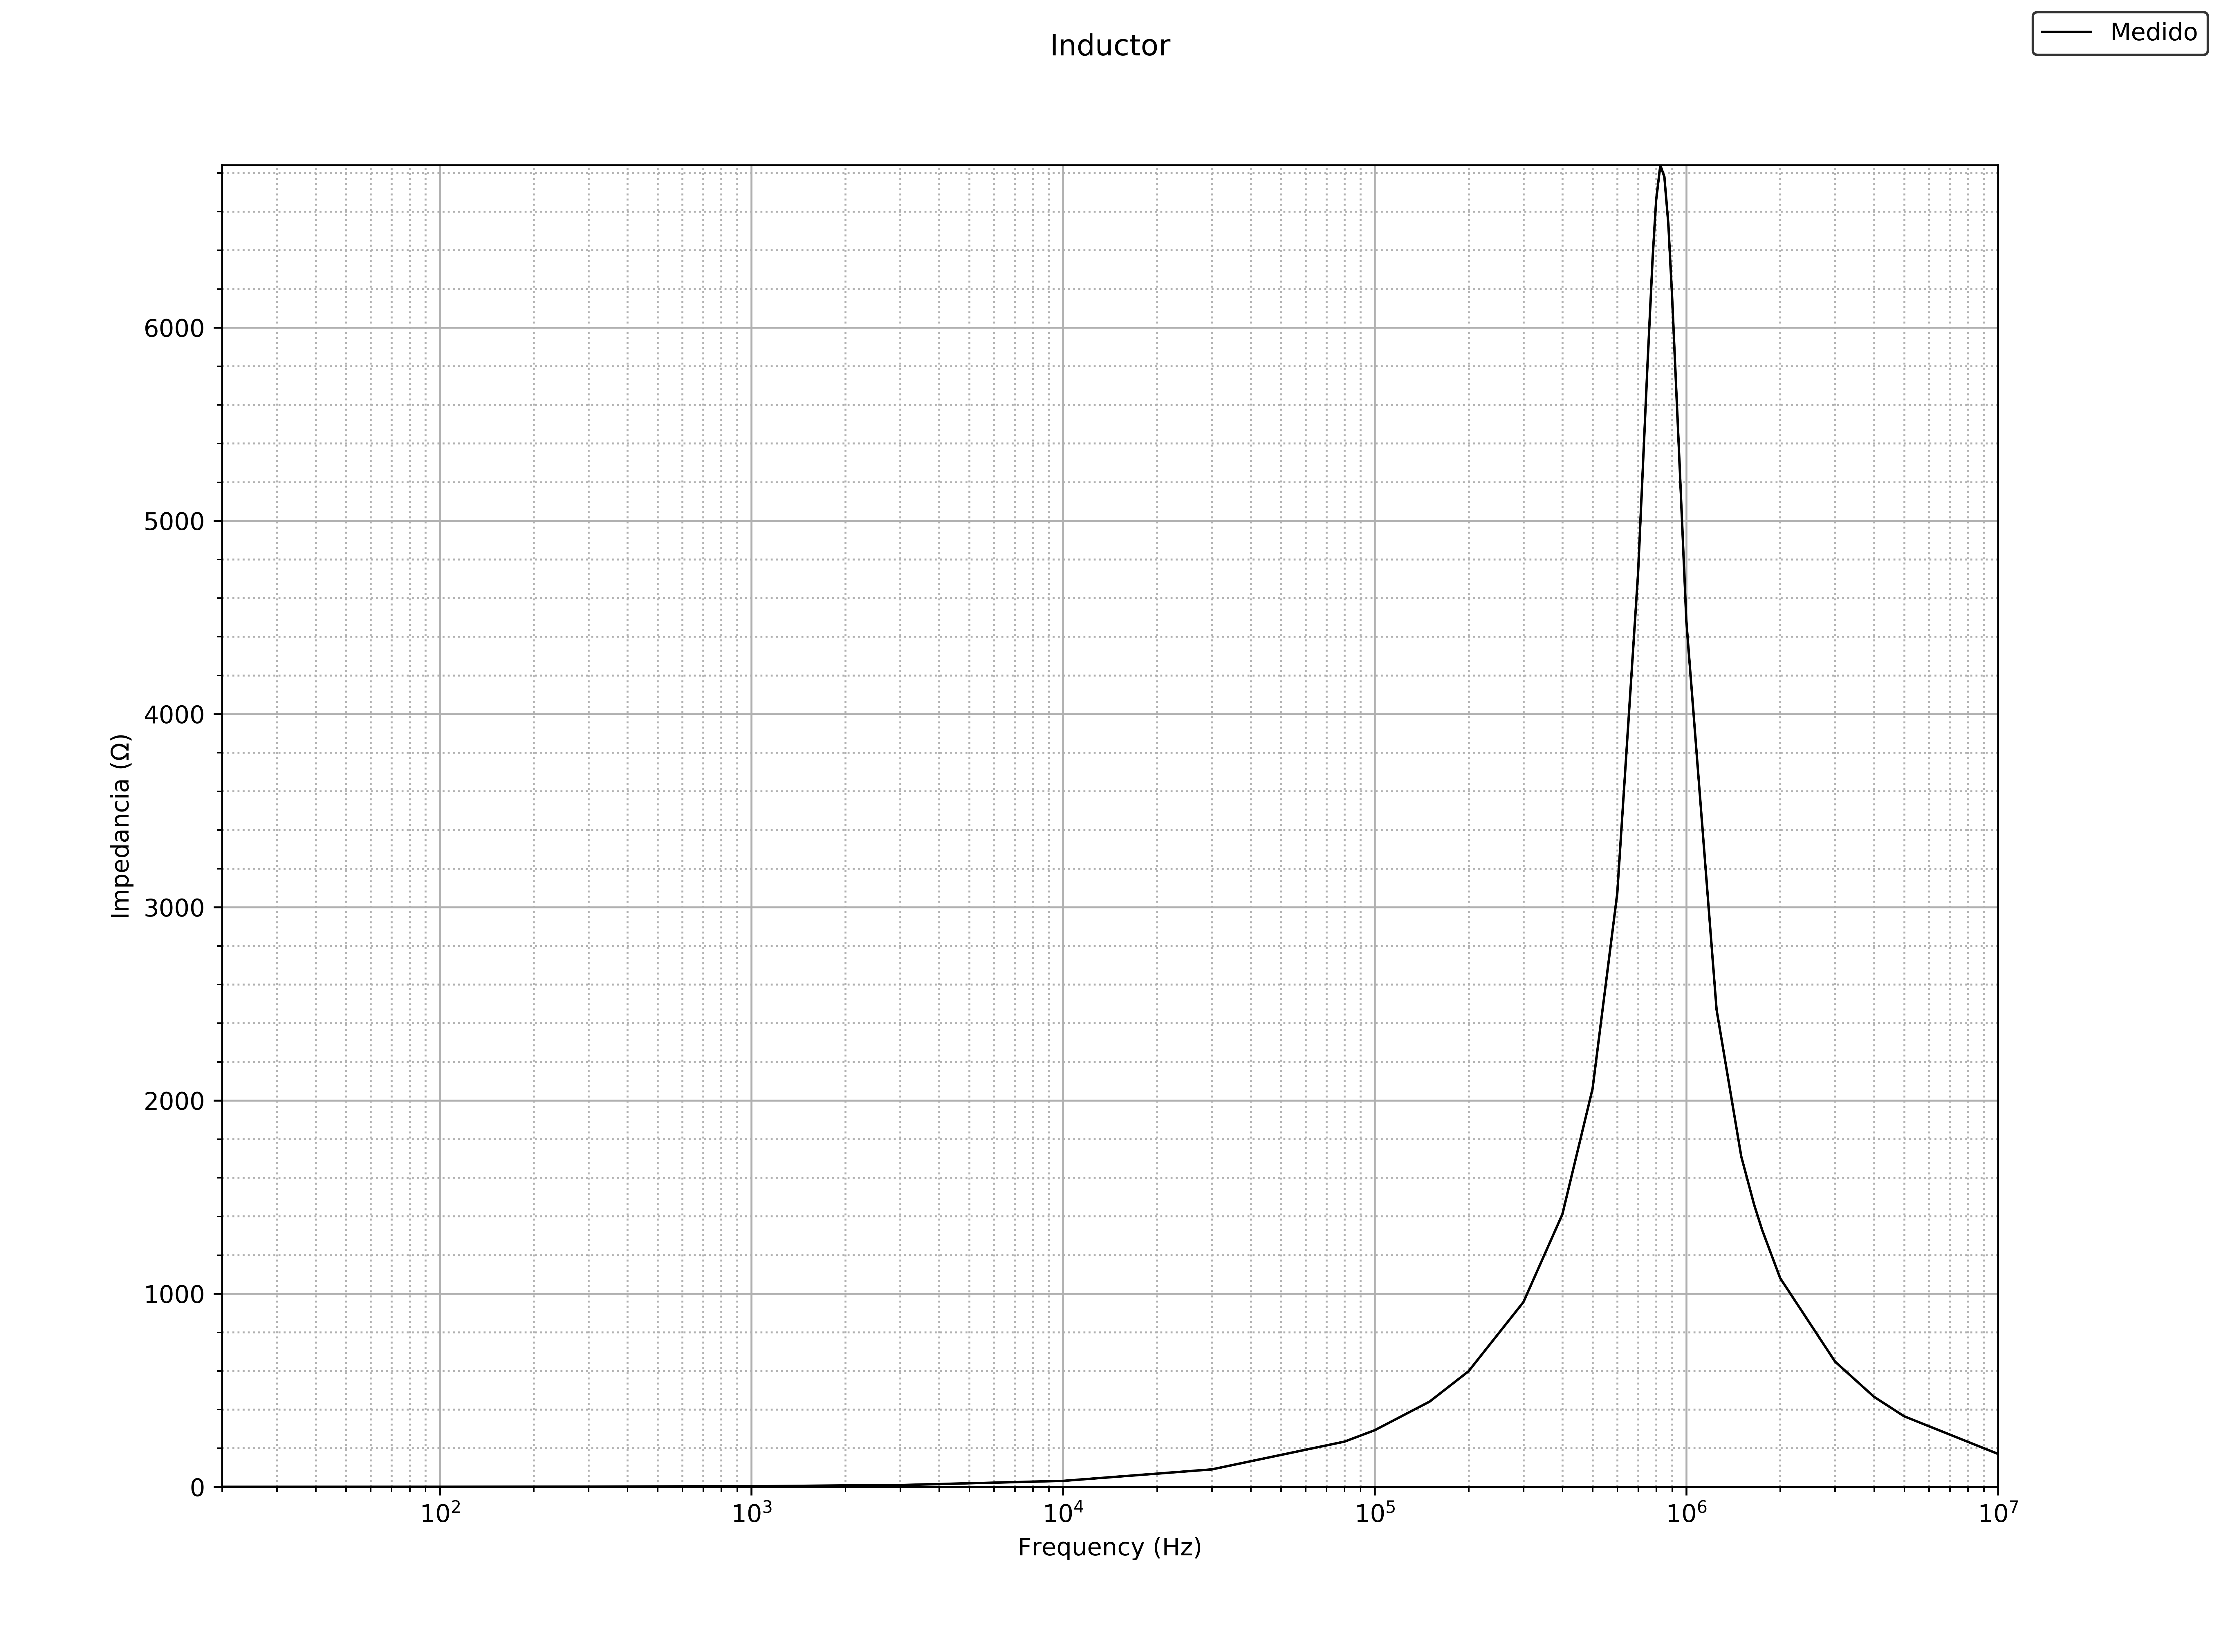
\includegraphics{Recursos/impedancia_medida_ind.png} &
            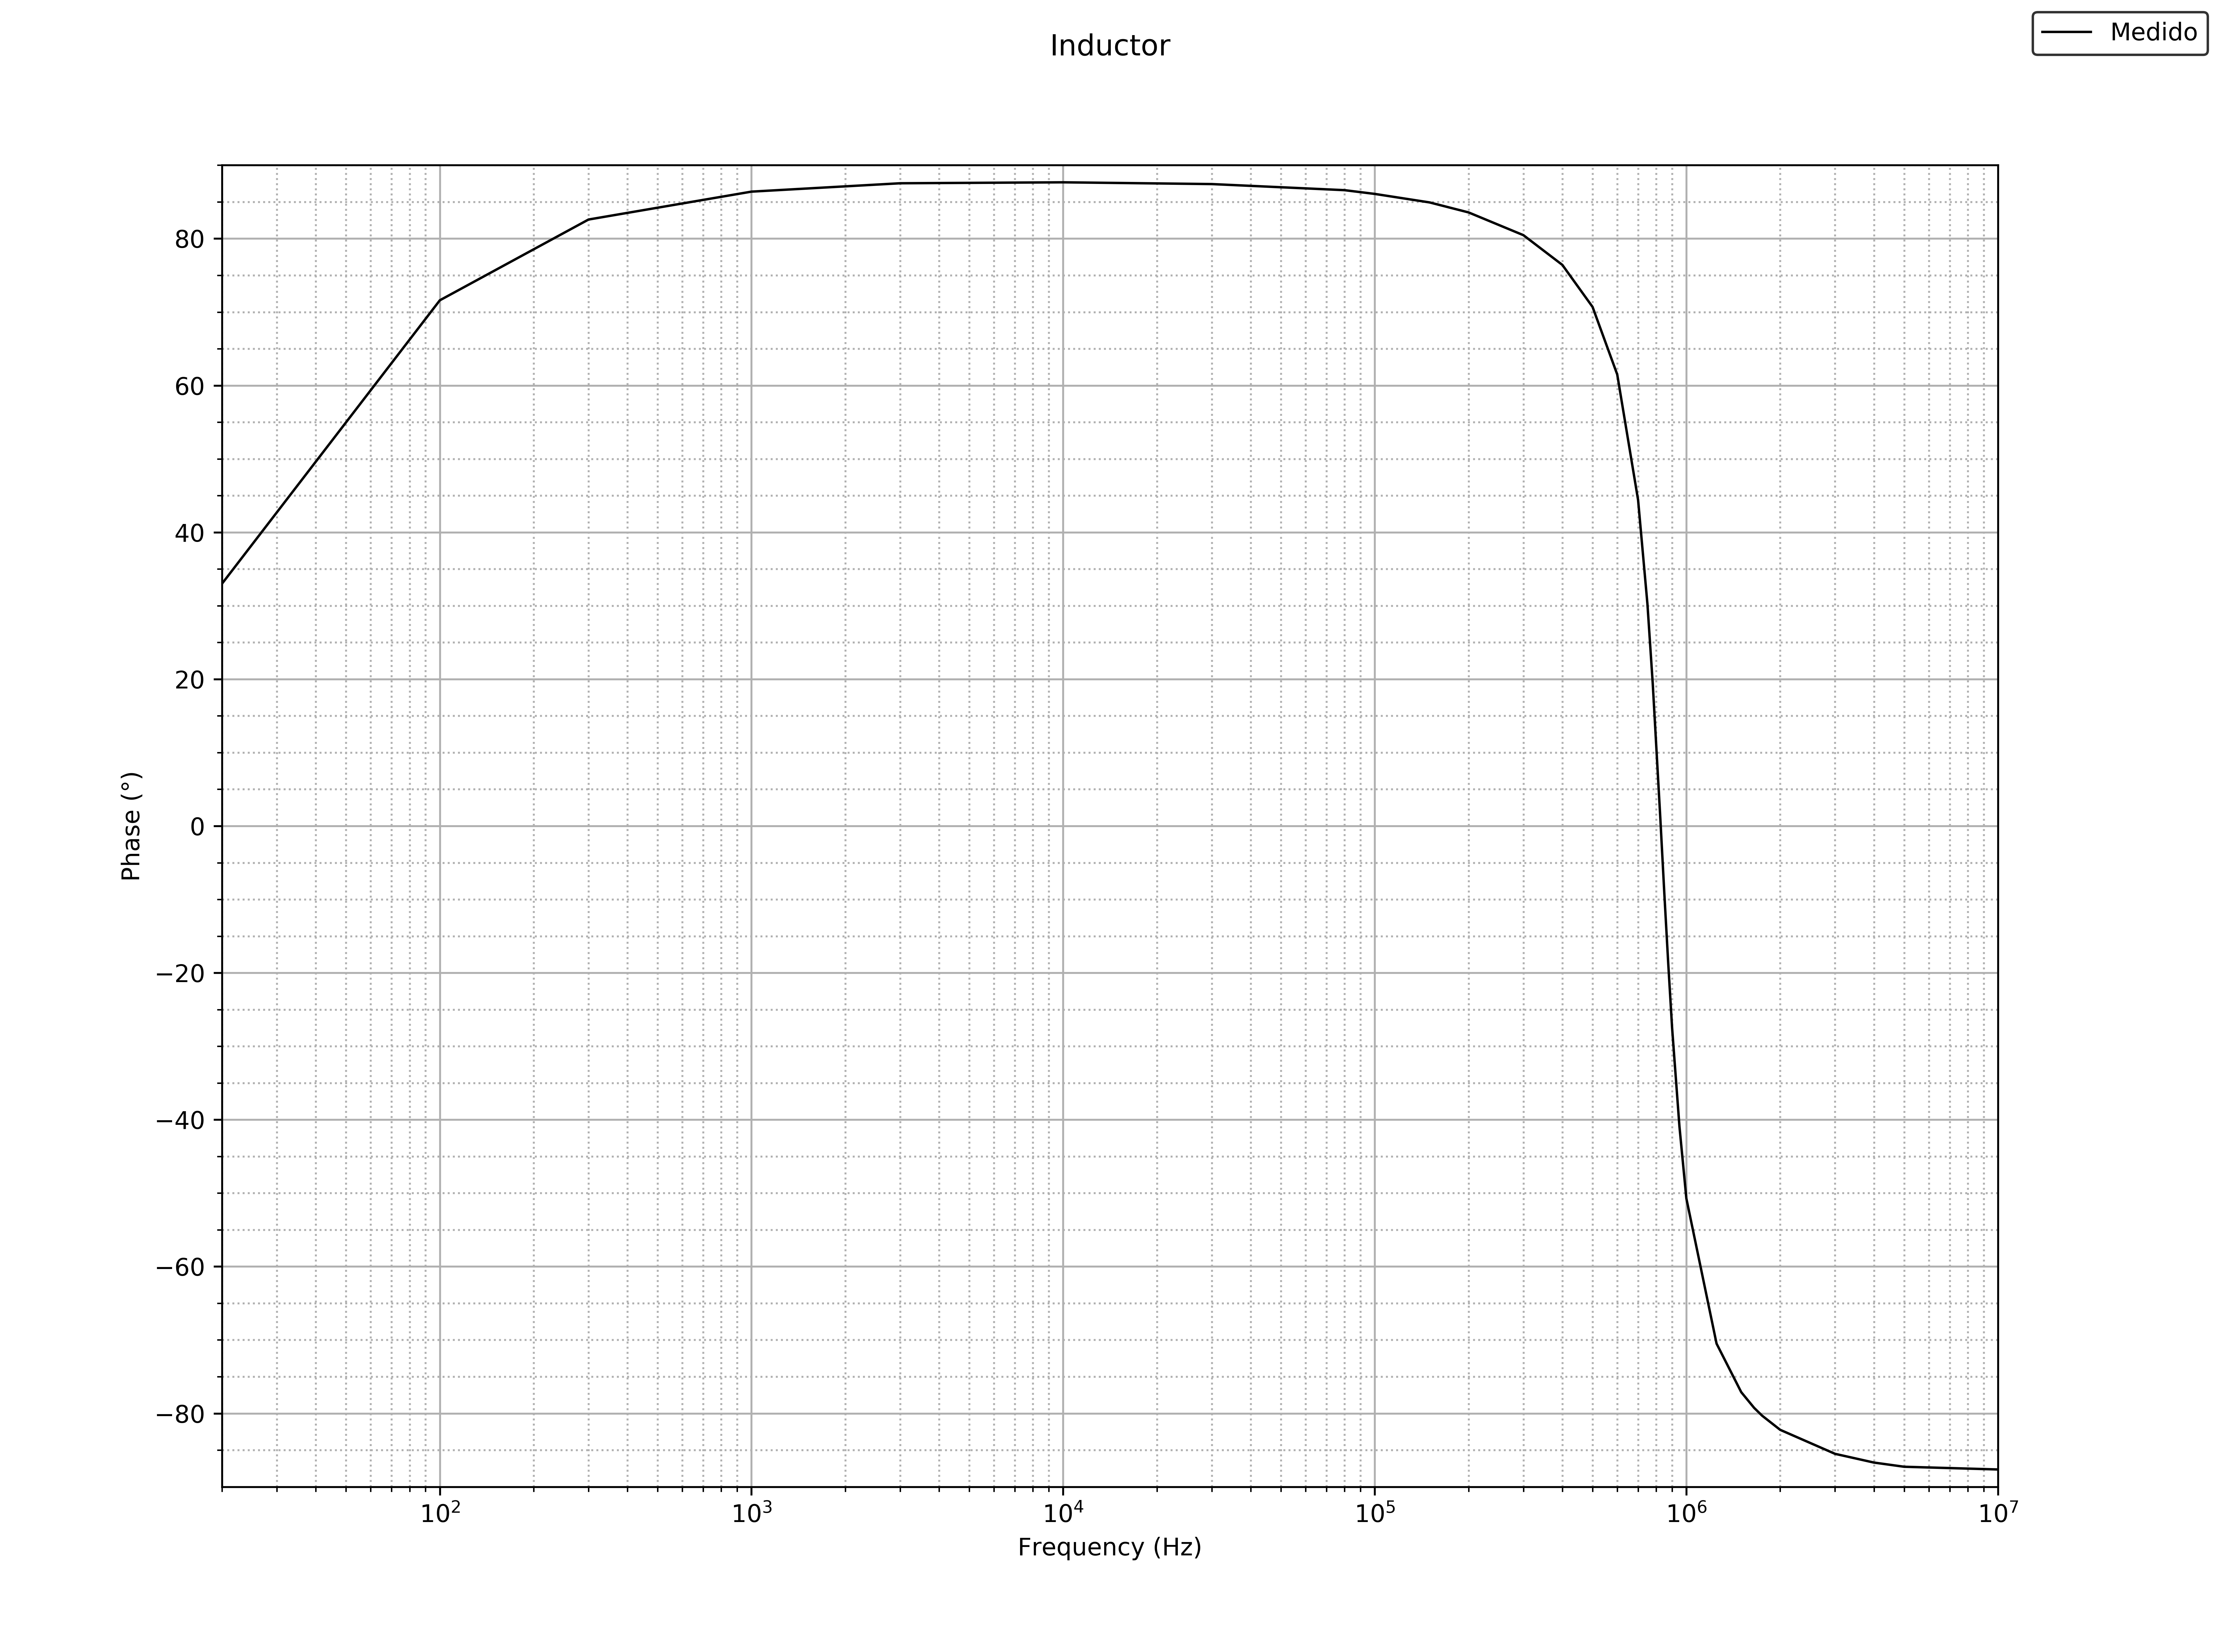
\includegraphics{Recursos/fase_medida_ind.png}

        \end{tabular}
    }
    \caption{Gr\'aficos realizados a partir de las mediciones}
    \label{fig:Med_IND}
        
\end{figure}    

\subsubsection{Modelizaci\'on del comportamiento observado}
Se propone el circuito de la Figura \ref{fig:modelo_IND} con el fin de encontrar un modelo que se ajuste al comportamiento real del inductor tanto en impedancia como en fase.
\begin{figure}[H]
    \centering
    \resizebox{0.5\textwidth}{!}{
        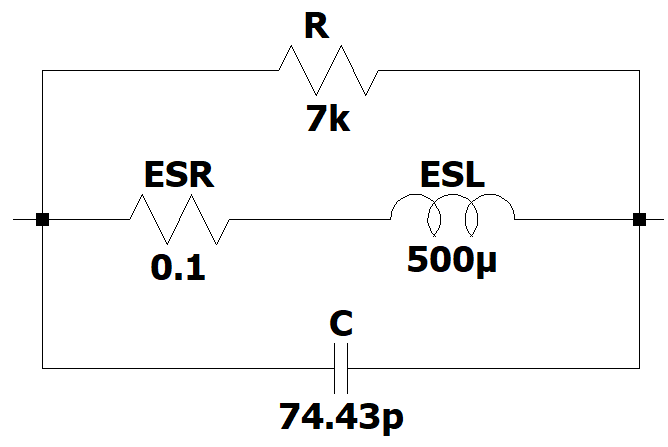
\includegraphics{Recursos/Modelo_ind.png}
    }
    \caption{Modelo de comportamiento del inductor}
    \label{fig:modelo_IND}
\end{figure}
Asumiendo que el valor de la inductancia es de $500\mu Hy$, lo cual es correcto si se tiene en cuanta que para frecuencias medias ese es el valor que se obtuvo en las mediciones, se puede encontrar un valor para $C$ de igual forma que para el modelo del capacitor y tomando el valor para la frecuencia de corte $f_0 = 825KHz$ que nuevamente es el valor para el cual la inductancia medida con el analizador de impedancias pasa de positiva a negativa.

Para los valores de $ESR$ y $R$ se eligen valores de manera que para frecuencias bajas la resistencia equivalente del modelo coincida con la impedancia medida, y se fija el valor $R = 7K\Omega$ para lograr un mejor ajuste a la curva medida, limitando la m\'axima impedancia del modelo.

Se muestran en la Figura \ref{fig:Comp_IND}, los resultados obtenidos a partir del modelo elegido.
\begin{figure}[H]
    \centering
    \resizebox{\textwidth}{!}{
        \begin{tabular}{c c}
            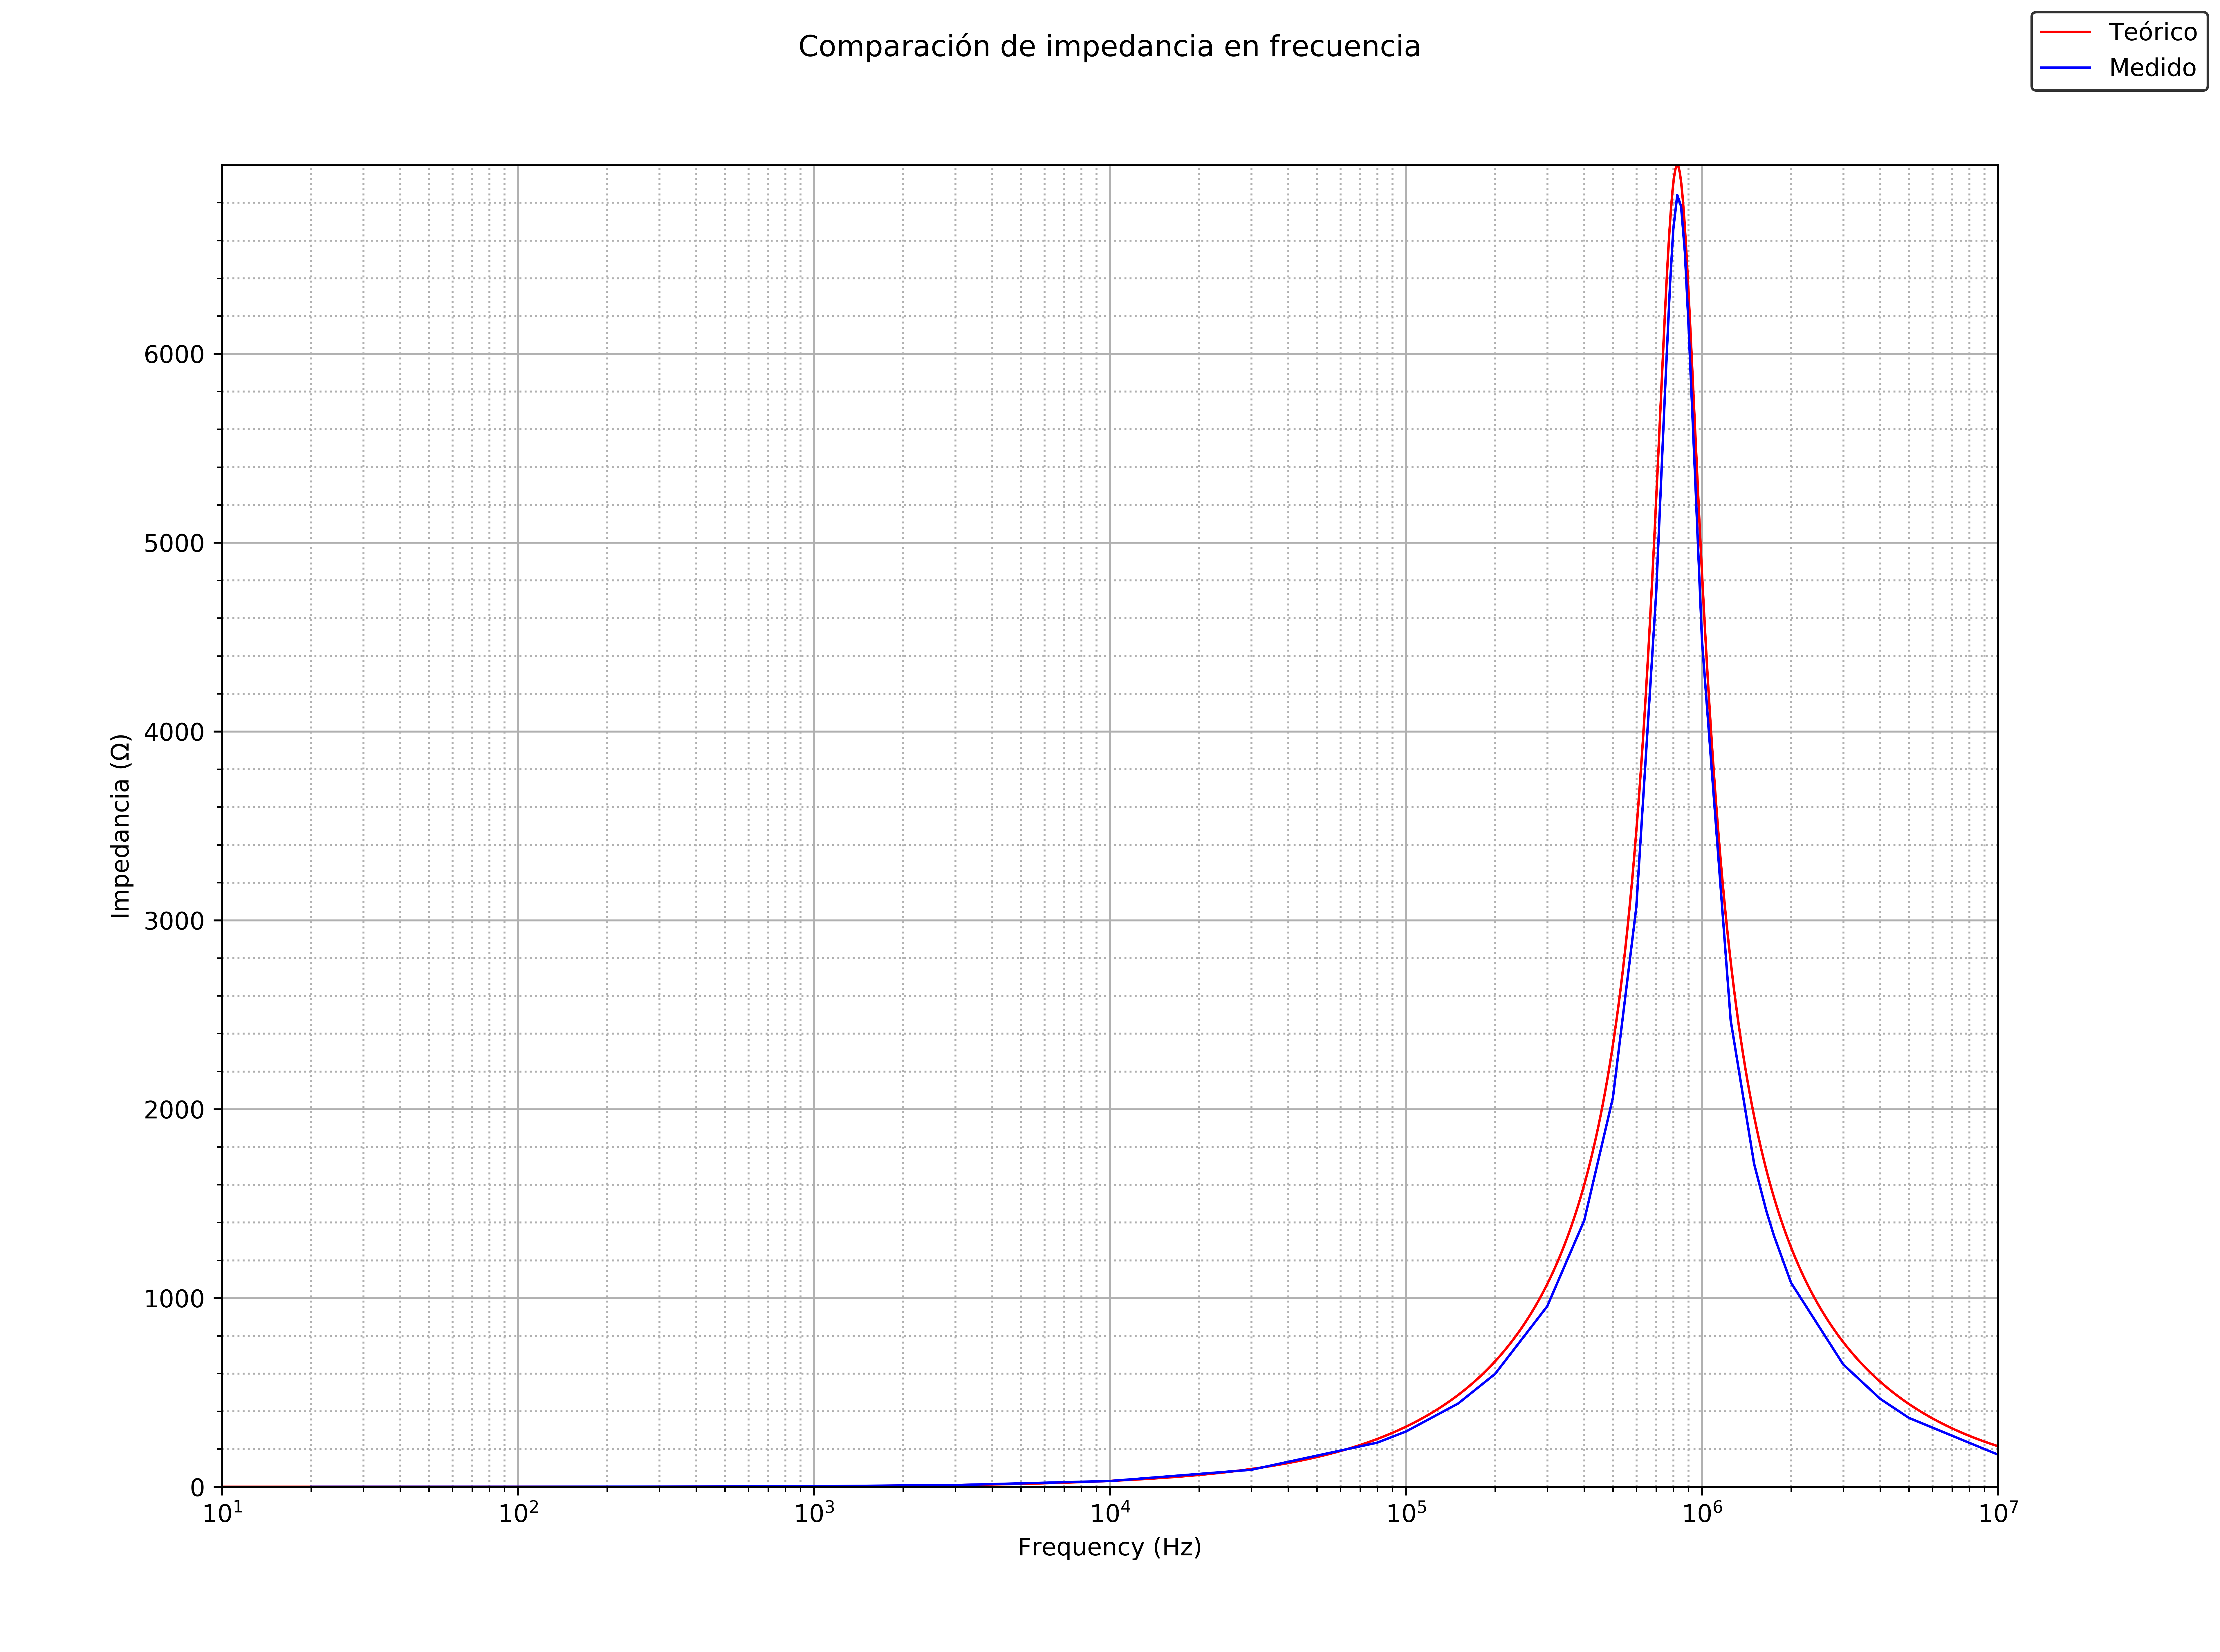
\includegraphics{Recursos/comp_impedancia_ind.png} &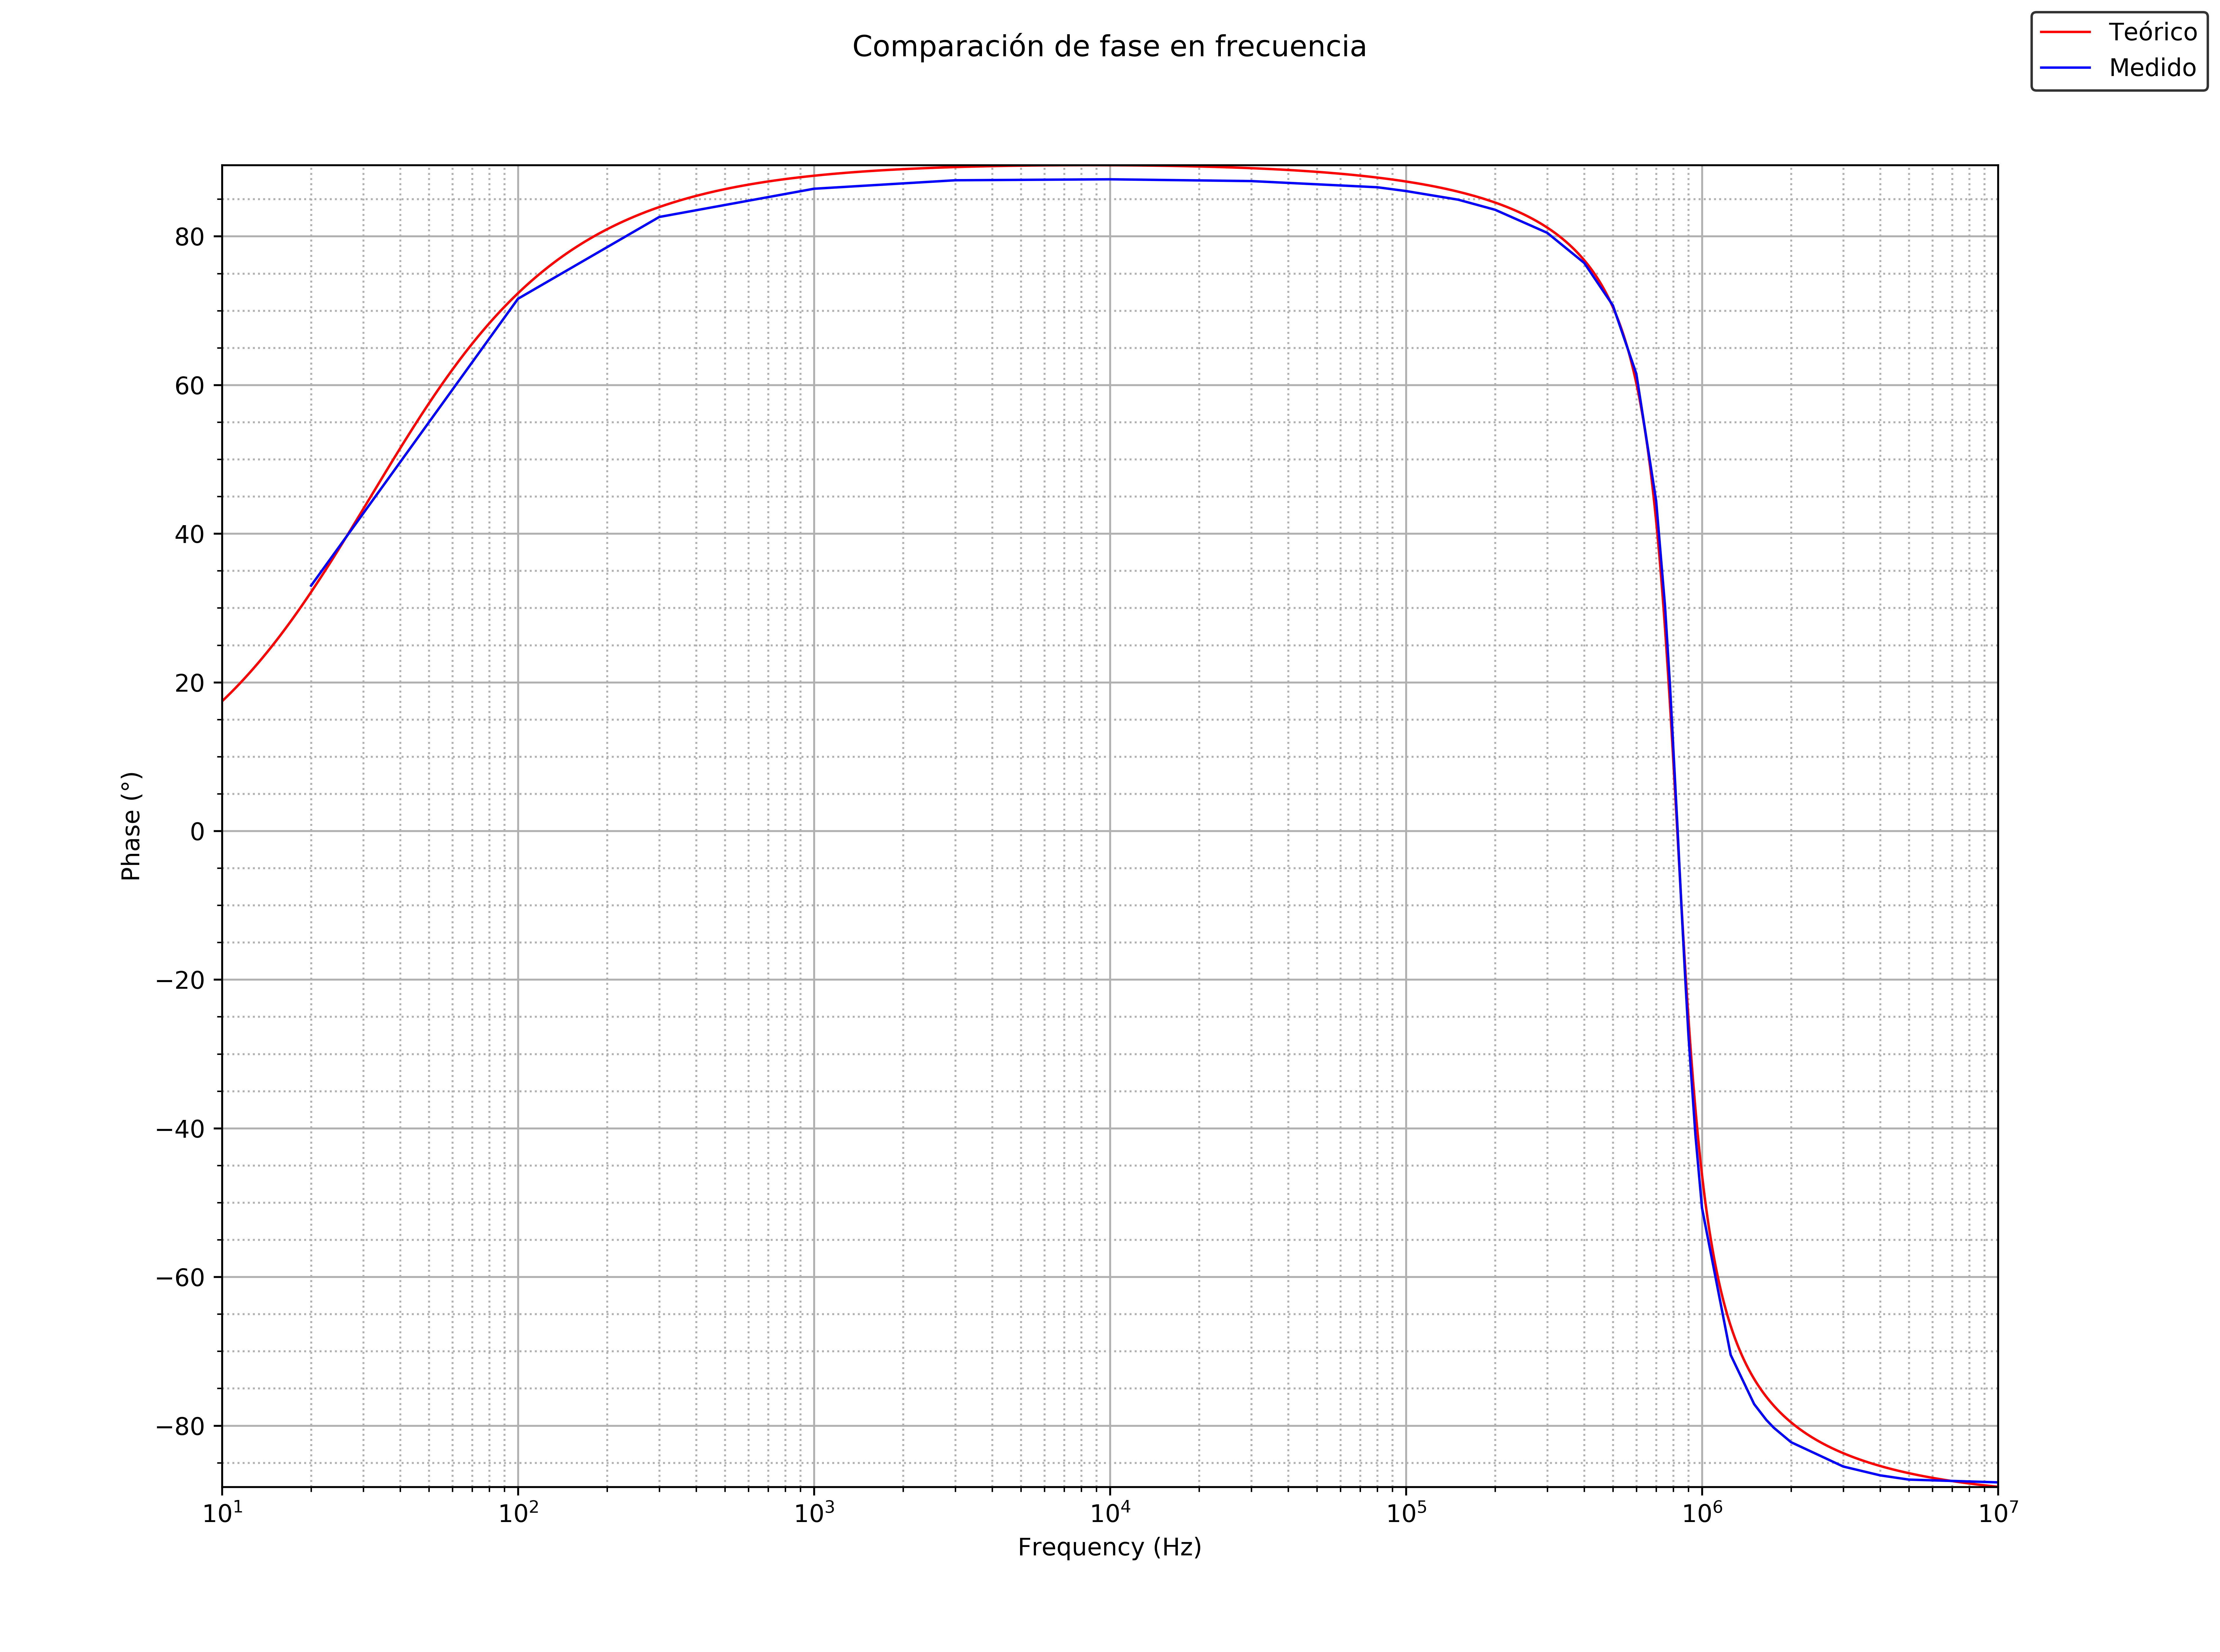
\includegraphics{Recursos/comp_fase_ind.png}
        \end{tabular}
        
    }
    \caption{Comparaci\'on entre mediciones y modelo de impedancia y fase en funci\'on de la frecuencia. }
        \label{fig:Comp_IND}    
\end{figure}

En este caso se observa un ajuste mucho mejor con las curvas medidas.


\subsection{Conclusiones}
Es posible observar en las distintas curvas mostradas en esta secci\'on, las variaciones que los componentes pasivos tienen con la frecuencia. 

Para una frecuencia fuera del rango de operaci\'on, un capacitor puede comportarse como un inductor y viceversa. Es por esto que es de suma importancia, al dise\~nar un circuito de apliaci\'on, elegir correctamente el modelo con el que se trabaja.
    \newpage
    
\section{2. Puente de Wien - Medici\'on de frecuencias}


El puente de Wien es un tipo de puente que consiste en dos capacitores y cuatro resistores. El mismo puede utilizarse para el cálculo de frecuencias lográndose la siguiente condición de balance:


\begin{figure}[H]
\begin{center}
\begin{circuitikz}
	
	\node [](Vg){}; 
	\draw (Vg) to[american voltage source , l = $V_g$] ++(0, -6) to[short] ++(4.5, 0);	
	\draw (Vg) to[short] ++(1.5, 0) node[](begin){} to[C, l =$C_1$] ++(0, -1.5) to[R, l = $R_1$] ++(0, -1.5) node[](vdl){};
	\draw (vdl) to[short] ++(0, -0.5) node[](parallel){};
	\draw (parallel) to[short] ++(1.25,0) to[R, l = $R_3$] ++(0, -2) to[short] ++(-1.25,0);
	\draw (parallel) to[C, l = $C_3$] ++(0, -2) to[short] ++(0, -0.5) node[ground]{};
	
	\draw (begin) to[short] ++(3,0) to[R, l = $R_2$] ++(0, -3) to[R, l = $R_4$] ++(0, -3);
	\draw (vdl) to[short] ++(3,0);
	

\end{circuitikz}
	\caption{Puente de Wien}
	\label{fig:Wien}
\end{center}
\end{figure}

\begin{equation}
f = \frac{1}{2\pi\sqrt{R_1R_3C_1C_3}}
\end{equation}

Para el caso en el que $R_1 = R_3$ y $C_1 = C_3$ la igualdad se simplifica:

\begin{equation}
f = \frac{1}{2\pi RC}
\end{equation}

con $R$ y $C$ el valor de los componentes.


En general se busca ajustar los valores de $R_1$ y $R_3$ para que coincidan y as\'i se cumpla la condici\'on de puente.

Asimismo se debe considerar $R_2 = 2 \cdot R_4$ para que se cumpla dicha condici\'on.

%%agregar aca sensibilidades 
\subsection{Diseno y elecci\'on de componentes}

Los componentes fueron seleccionados realizando c\'alculos para que el puente pueda estabilizarse en el rango de frecuencias solicitado ($100Hz$ a $2KHz$). De esta forma se tiene la siguiente distribuci\'on, tomando en cuenta las suposiciones realizadas con anterioridad.

\begin{table}[H]
    \centering
    \begin{tabular}{c c c c}
        $C_1 = C_3$ & $R_2 = 2 \cdot R_4$ & $R_1 = R_3 (preset)$ \\
        \hline \\
        $33 nF$ & $10 K\Omega$ & $50 K\Omega$ \\
        \hline
    \end{tabular}
\end{table}

Cabe destacar que se consider\'o un cierto margen en el rango de frecuencias, teniendo en cuenta las tolerancias de los componentes.



\subsubsection{Sensibilidades}
Se calcul\'o la sensibilidad del puente respecto a los componentes que se eligi\'o variar ($R_1$ y $R_3$).

La sensibilidad respecto de $R_1$ se puede calcular como:

\begin{equation}
\Delta V_d = \frac{Z_3 \cdot (Z_2+Z_4) - Z_4(Z_1 + \Delta Z_1 + Z_3)}{(Z_1+Z_3) \cdot (Z_2+Z_4)} \cdot v_g
\end{equation}
 
Veamos que

\begin{equation}
\frac{|\Delta Z_1|}{|Z_1|} = \frac{\Delta R_1}{|Z_1|} = \frac{\frac{\Delta R_1}{R_1}}{\sqrt{1+\frac{1}{(\omega \cdot C_1 \cdot R_1)^2}}}
\end{equation}

Suponiendo $\frac{1}{\omega \cdot C_1 \cdot R_1} >> 1$ obtenemos:

\begin{equation}
\frac{|\Delta Z_1|}{Z_1} = \frac{|\Delta R_1|}{R_1} \cdot \omega \cdot C_1 \cdot R_1
\end{equation}


Sabiendo esto, y asumiendo condici\'on de puente y $v_g$ unitario obtenemos

\begin{equation}
\Delta V_d = \frac{-A}{(A+1)^2} \cdot \omega \cdot R_1 \cdot C_1 \cdot \frac{\Delta R_1}{R_1}
\end{equation}

Donde $A = \frac{R_2}{R_4}$ es el factor cabeza de puente, y esta relaci\'on fue fijada con anterioridad. 

Asumiendo los valores de la tabla de selecci\'on de componentes, se grafica la sensibilidad para el rango de frecuencia.

\begin{figure}[H]
    \centering
    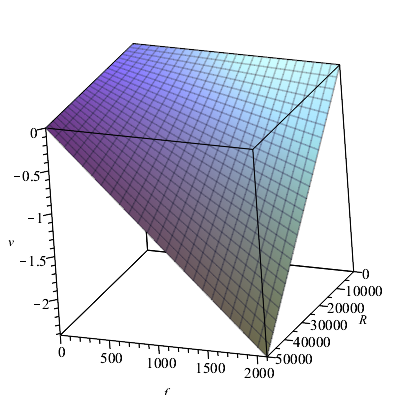
\includegraphics[width=0.9\textwidth]{Recursos/sensib_R1.png}
	\caption{Sensibilidad del circuito respecto a $R_1$}
   	\label{fig:sensib_R1}
\end{figure}

Se realiza un procedimiento an\'alogo para obtener la sensibilidad del puente respecto a $R_3$.

Veamos que:

\begin{equation}
Z_3 + \Delta Z_3 = \frac{R_3 + \Delta R_3}{1+S \cdot C_3 \cdot (R_3 + \Delta R_3)} 
\end{equation}

Suponemos $R_3 >> \Delta R_3$ y despreciamos los efectos de $\Delta R_3$ sobre el denominador debido a que est\'a multiplicado por un n\'umero relativamente peque\~no para el rango de frecuencias.

Luego se tiene

\begin{equation}
Z_3 + \Delta Z_3 = \frac{R_3}{1+S \cdot C_3 \cdot R_3} + \frac{\Delta R_3}{1+S \cdot C_3 \cdot R_3} = Z_3 + \frac{\Delta R_3}{1+S \cdot C_3 \cdot R_3}.
\end{equation}

Por lo que $\Delta Z_3 = \frac{\Delta R_3}{1+S \cdot C_3 \cdot R_3}$

Operando, se llega a la siguiente equivalencia:

\begin{equation}
\frac{|\Delta Z_3|}{|Z_3|} = \frac{\Delta R_3}{R_3}
\end{equation}

Finalmente, considerando $V_g$ unitario,

\begin{equation}
\Delta V_d = \frac{A}{(A+1)^2} \cdot \frac{\Delta R_3}{R_3}
\end{equation}

Por lo que ser\'a constante independientemente de la frecuencia ($V_d = \frac{2}{9}$).


\subsection{Mediciones}

Para la medici\'on del puente se utiliz\'o el mult\'imetro de banco. Con el mismo es posible medir niveles de tensi\'on que ser\'ian indistinguibles del ruido en un osciloscopio. Se estimul\'o al circuito con una senal de $5V_{pp}$ y se ajustaron los dos potensi\'ometros hasta obtener la menor tensi\'on posible:


\begin{table}[H]
\centering
\begin{tabular}{lllll}
Frecuencia del generador & Preset R\_1(Ohm) & Preset R\_2(Ohm) & Frecuencia calculada & Error(\%) \\ \hline
100                      & 46100            & 45915             & 104.83              & 3,92      \\
500                      & 9390             & 9175             & 519,6             & 4,83      \\
750                      & 6283             & 6219             & 771,55               & 2,87      \\
1000                     & 4695             & 4689             & 1027,89              & 2,79      \\
1250                     & 3833             & 3762             & 1270                 & 1,61      \\
1500                     & 3144             & 3125             & 1538,65              & 2,58      \\
1750                     & 2704             & 2665             & 1795,6               & 2,66      \\
2000                     & 2331             & 2318             & 2074,8               & 3,74     \\ \hline
\end{tabular}
\end{table}

En primer lugar se observa el comportamiento esperado respecto a las resistencias, para medir una frecuencia más cercana al límite inferior de la escala propuesta se precisan resistencias mayores. Además de lo anterior es importante hacer notar que el balance se logra solamente cuando ambos potenciómetros poseen resistencias casi iguales. Este balance no fue ideal, ya que no pudo llegarse a una diferencia de potencial igual a 0 entre ambas ramas, en cambio se tomó como $0$ el menor valor posible dada la frecuencia medida. Dicha tensión fue siempre menor a $10mV$. Dado el voltaje con el que se estimuló al circuito y el error porcentual obtenido  puede cdecirse que los resultados son satisfactorios y queda poco lugar para mejoras. Incluir las resistencias equivalentes de los capacitores utilizados tanto como las capacitancias parásitas de las resistencias es una de esas mejoras. No obstante, dadas las frecuencias en las que se trabajó, las capacitancias y las resistencias parásitas son despreciables en comparación a las tolerancias reales de los componentes. 




\subsection{Conclusiones}

Como conclusi\'on se puede destacar que se notaron diferencias entre el modelo te\'orico del puente y las mediciones realizadas en la pr\'actica. Principalmente se observa que es muy dificil equilibrar el puente en su totalidad, debido a las variaciones en los presets de ajuste y las tolerancias asociadas a los componentes del circuito.
    \newpage
    \section{4. Modulaci\'on de se\~nal con FM}
La modulci\'on FM consiste en utilizar una señal modulante para variar la frecuencia de la señal portandora alrededor de la frecuencia portadora en un rango espec\'ifico. Puede definirse al igual que en modulaci\'on AM un coeficiente de modulaci\'on , el cual representa la desviaci\'on de frecuencia m\'axima como multiplo de la m\'axima frecuencia de la moduladora. Para este ejercicio se repitieron los puntos $b$, $c$ y $d$ del inciso anterior para una modulaci\'on FM. 


\subsection{Mediciones}
A continuaci\'on se dejan los espectros obtenidos:


\begin{figure}[H]
    \centering
    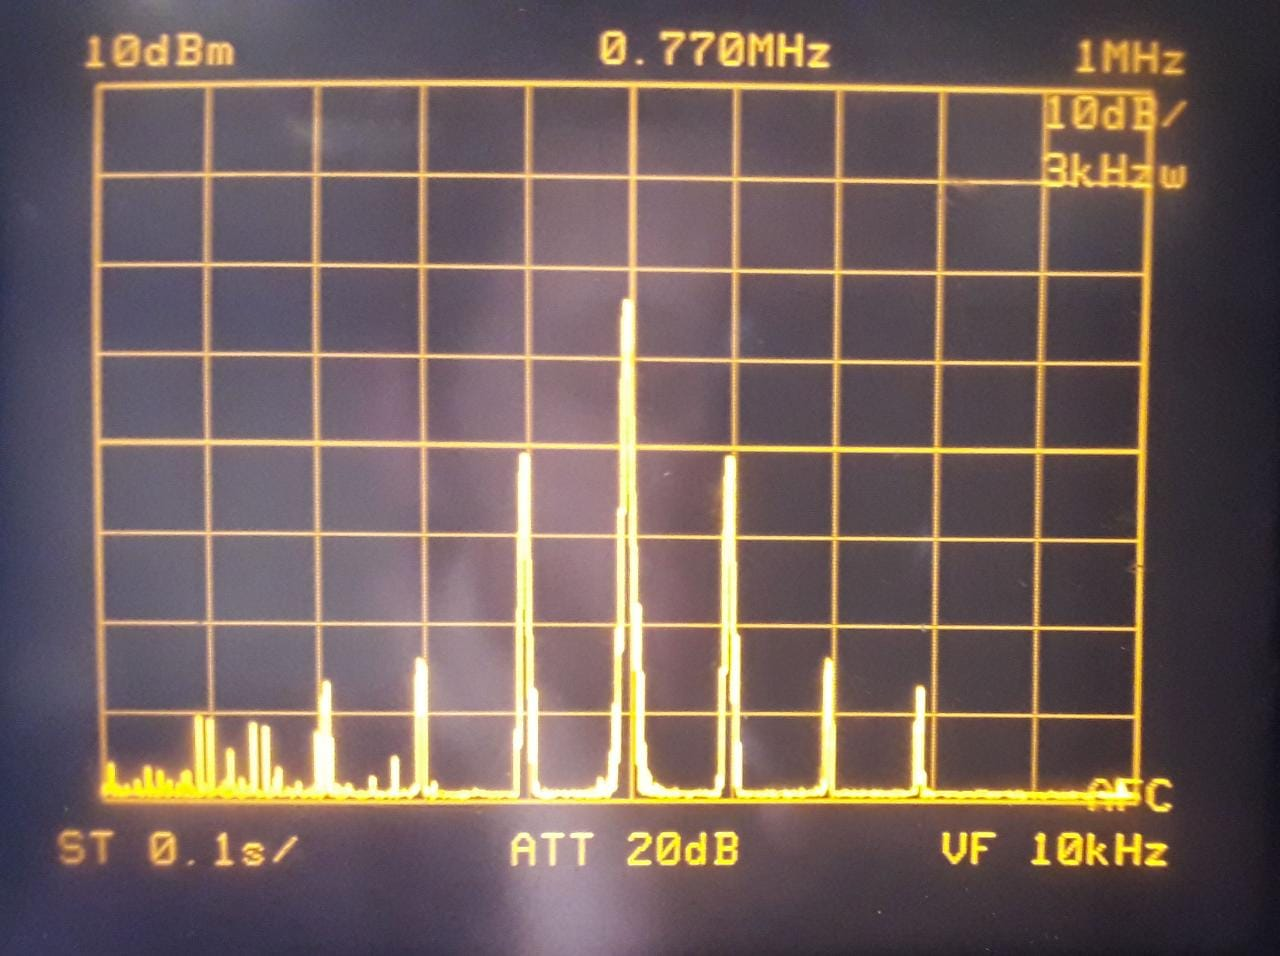
\includegraphics[scale=0.3]{Recursos/Ej4_senoidal.jpeg}
    \caption{Espectro señal senoidal con $m = 0.5$}
\end{figure}\label{fig:espectro1}

\begin{figure}[H]
    \centering
    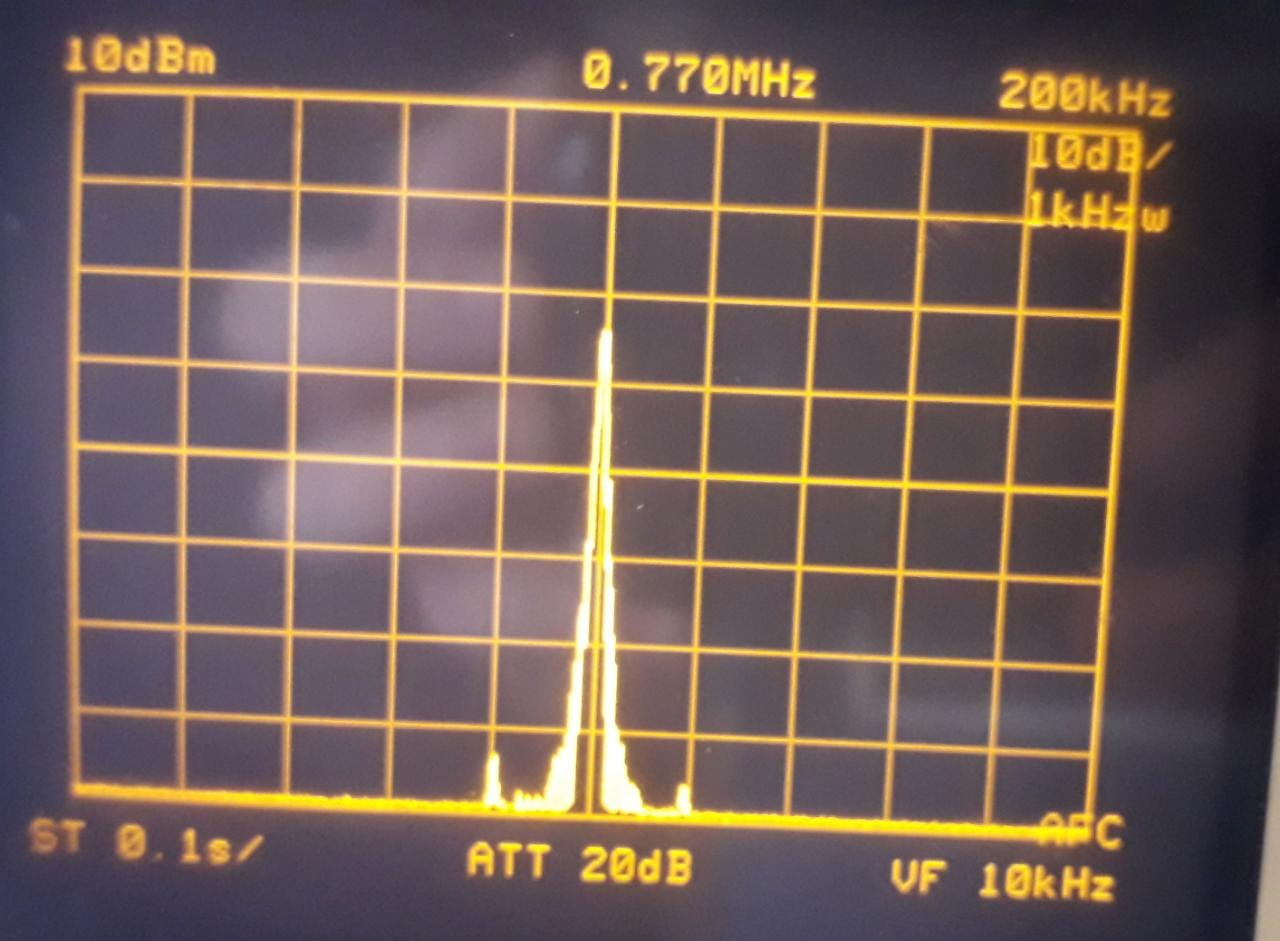
\includegraphics[scale=0.3]{Recursos/Ej4_senoidal_800K.jpeg}
    \caption{Espectro señal senoidal con frecuencia portadora}
\end{figure}

\begin{figure}[H]
    \centering
    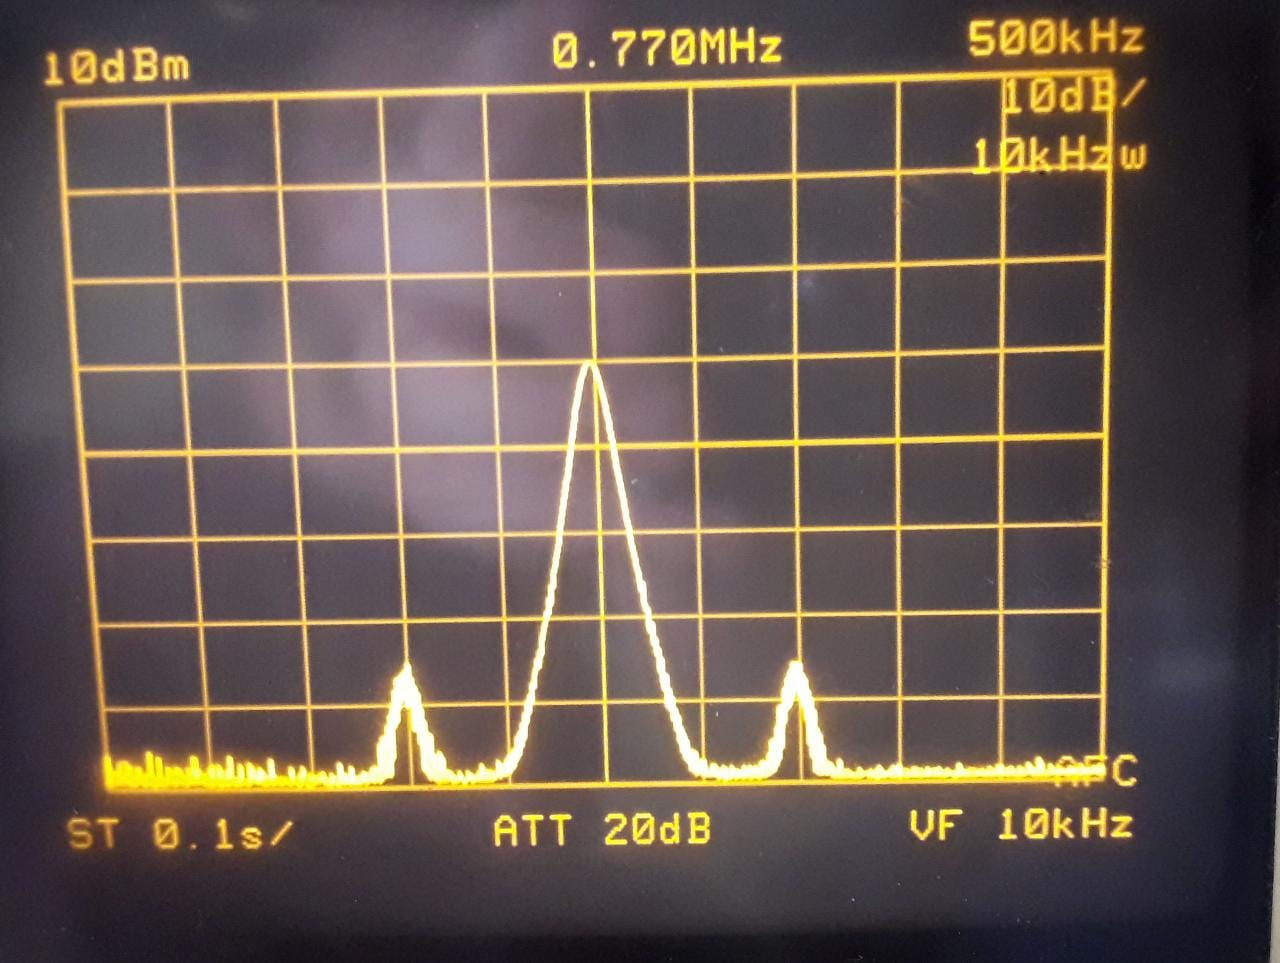
\includegraphics[scale=0.3]{Recursos/Ej4_triangular_m1.jpeg}
    \caption{Espectro señal triangular con $m = 1$}
\end{figure}


\subsection{An\'alisis de los resultados}

Debido a que en la modulación FM se hace variar la frecuencia de la portadora se esperaría ver ese comportamiento reflejado en forma de armónicos en el analizador de espectros. En la figura \ref{fig:espectro1} se ve claramente lo anterior, en el centro, nuevamente desvíada en $30kHz$ está la frecuencia fundamental, y alrededor de ella se ven 3 pares de armónicos distanciados de manera proporcional, por lo que se cumple la hipótesis incial de modulación FM. Para el caso en el que las frecuencias de las dos señales son iguales ocurre lo mismo que en el ejercicio anterior, y no hya armónicos presentes. Para la triangular, la explicación es análoga al ejercicio 3.


    \newpage
    \myexternaldocument{ej2}
\myexternaldocument{ej4}

\section{Medici\'on de factor de calidad}
\subsection{Filtro Pasabajos}
\label{sec:FPB}
Se puede observar en la Figura \ref{eq:Trans_PB} que, al reemplazar en la tranferencia a $s$ por $j\omega _0$ se obtiene que $H(s) = \frac{-j}{2\xi} = -j\cdot Q $. Por lo tanto, al calcular el m\'odulo de la trasferencia se puede conocer un valor para el $Q$ del circuito.


En este caso, para obtener un valor para la frecuencia de corte se selecciona, de las mediciones del la variaci\'on de fase en funci\'on de la frecuencia en la Figura \ref{fig:respuesta_frecuencia_pasabajos}, el valor que genera una diferencia de fase de $-90^{\circ}$. Ese punto se corresponde con una frecuencia de $48.9KHz$ y para esa frecuencia el modulo de la trasferencia es de $0.874dB$. 
Se calcula luego, como se muestra en \ref{eq:calc_q_PB}, un valor para $Q$ pasando ese valor a veces.
\begin{equation}
    Q = 10^{\frac{|H(S)|_{dB}}{20}}
    \label{eq:calc_q_PB}
\end{equation}
Se obtiene para este circuito que $Q = 1.105$. Al compararlo con el valor te\'orico calculado como $Q = \frac{1}{2 \cdot \xi} = 1.25$ se observa un error del 11\%, que se encuentra dentro de lo esperado.

\subsection{Filtro Pasaaltos} 

Para este circuito se vuelve a aplicar el m\'etodo utilizado en la Secci\'on \ref{sec:FPB}.
Se reemplaza en \ref{eq:trans_PA} y se obtiene un valor para $Q$ reemplazando la frecuencia de corte del circuito de $f_0 = 46.2KHz$ en \ref{eq:calc_q_PB}.
Se obtiene para este circuito que $Q = 1.04$. Al compararlo con el valor te\'orico calculado como $Q = \frac{1}{2 \cdot \xi} = 1.25$ se observa un error del 17\%, que nuevamente se encuentra dentro de lo esperado.


\subsection{Filtro Pasabanda}
\label{sec:FPBa}
Se sabe que para un filtro pasabanda se puede calcular el $Q$ como se ve en \ref{eq:Q_formula}

\begin{equation}
    Q = \frac{\omega_0}{\Delta \omega}
    \label{eq:Q_formula}
\end{equation}

Adem\'as, es posible conocer el ancho de banda al medir los valores de frecuencia para los cuales la transferencia del sistema baja 3dB respecto de la banda pasante. Luego el valor absoluto de la resta de estas es el ancho de banda $\Delta \omega$. Para la frecuencia de corte nuevamente se observa la fase siguiendo el mismo procedimiento que los casos anteriores.

Se obtiene, al reemplazar en \ref{eq:Q_formula} el valor de la transferencia en la frecuencia de corte y del ancho de banda, $f_0 = 48Khz$ y $\Delta f_0 = 20KHz$ respectivamente, y sabiendo que $\omega = 2\pi \cdot f$, se obtiene que $Q = 2.25$. Al compararlo con el valor te\'orico calculado como $Q = \frac{1}{2 \cdot \xi} = 1.25$ se observa un error muy grande, esto se debe a que no se ajusto el 
$\xi$ como en las secciones anteriores, sino que se utiliz\'o una resistencia de $120\Omega$ y adem\'as, para este caso, se realizaron las mediciones antes del buffer. Por lo tanto, esta medici\'on no es correcta y el resultado no tiene sentido.  

\subsection{Filtro Rechazabanda}

Para este circuito se vuelve a aplicar el m\'etodo utilizado en la Secci\'on \ref{sec:FPBa}.
Se reemplaza en \ref{eq:Q_formula} el valor medido para la frecuencia de corte y el ancho de banda y se obtiene un valor para $Q = 1.04$.
 Al compararlo con el valor te\'orico calculado como $Q = \frac{1}{2 \cdot \xi} = 1.25$ se observa un error del 17\%. Sin embargo en estas mediciones tampoco se tuvo en cuenta la correcci\'on del $\xi$. A pesar de ello, los resultados se ajustan al te\'orico correctamente. 


\end{document}